\newpage
\section{深度迁移学习}

随着深度学习方法的大行其道,越来越多的研究人员使用深度神经网络进行迁移学习。对比传统的非深度迁移学习方法,深度迁移学习直接提升了在不同任务上的学习效果。并且,由于深度学习直接对原始数据进行学习,所以其对比非深度方法还有两个优势:\textit{自动化地提取更具表现力的特征},以及\textit{满足了实际应用中的端到端(End-to-End)需求}。

近年来,以生成对抗网络(Generative Adversarial Nets, GAN)~\cite{goodfellow2014generative}为代表的对抗学习也吸引了很多研究者的目光。基于GAN的各种变体网络不断涌现。对抗学习网络对比传统的深度神经网络,极大地提升了学习效果。因此,基于对抗网络的迁移学习,也是一个热门的研究点。

图~\ref{fig-deep}展示了近几年的一些代表性方法在相同数据集上的表现。从图中的结果我们可以看出,深度迁移学习方法(BA、DDC、DAN)对比传统迁移学习方法(TCA、GFK等),在精度上具有无可匹敌的优势。

\begin{figure}[htbp]
	\centering
	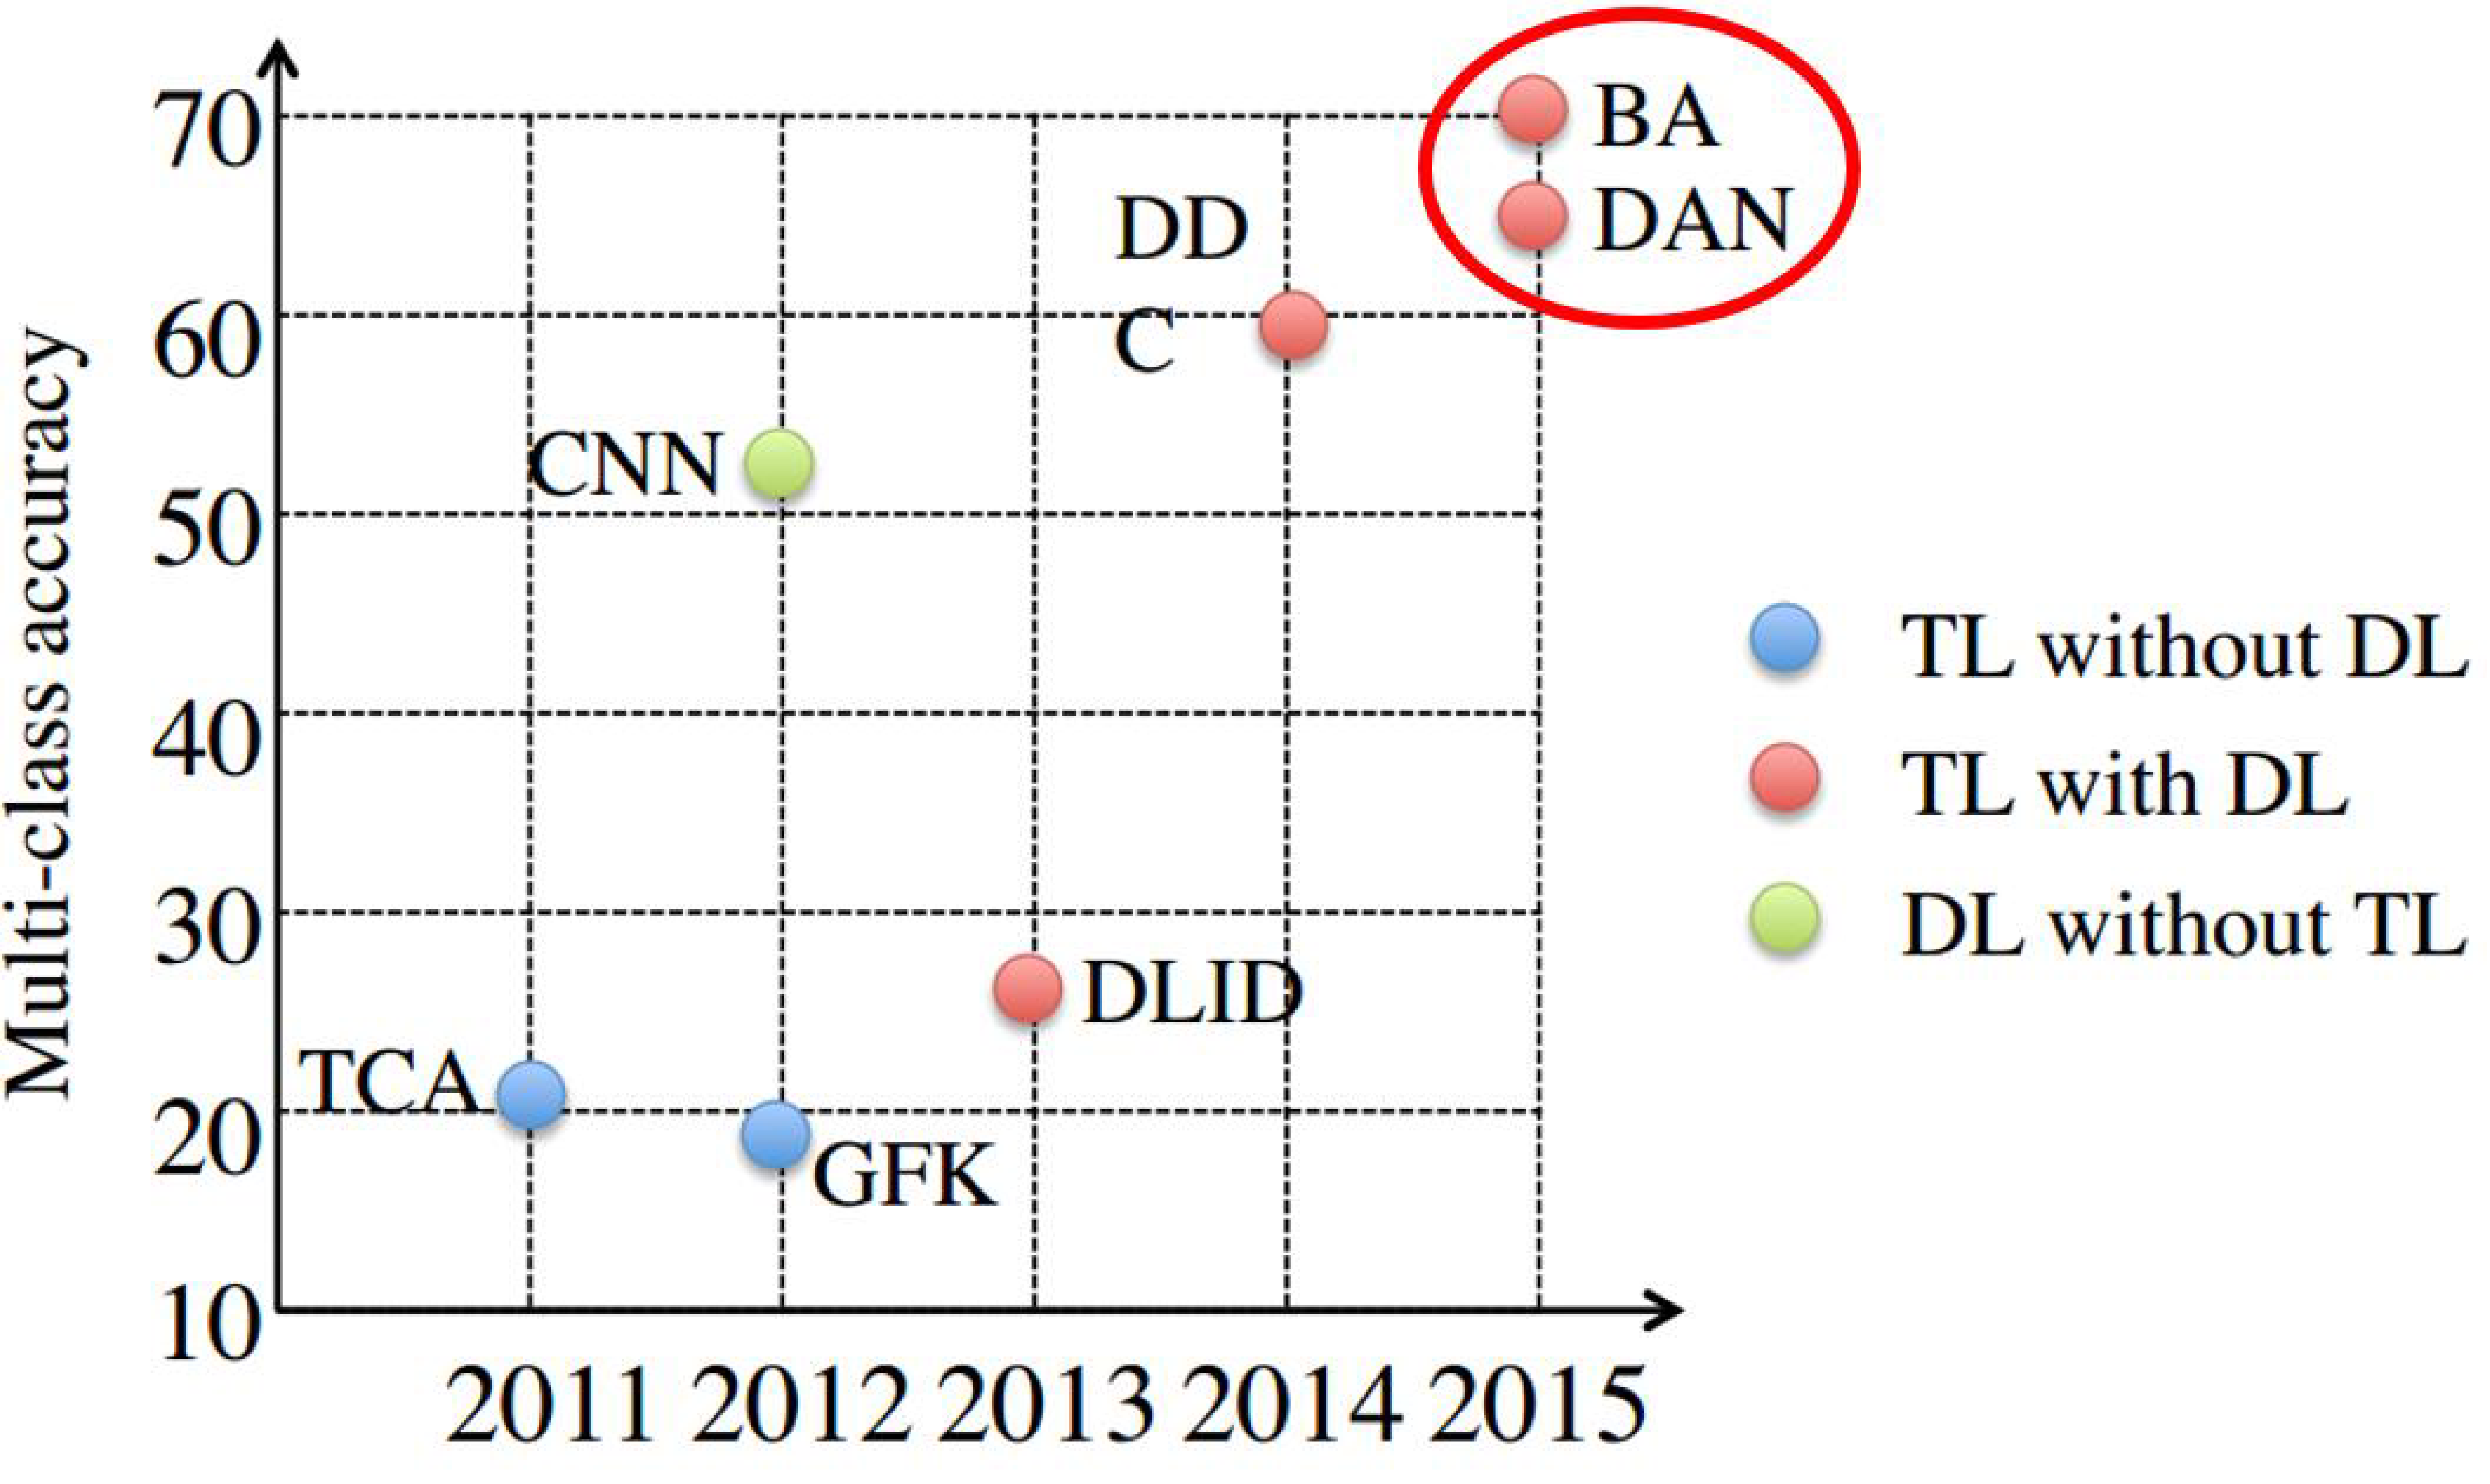
\includegraphics[scale=0.42]{./figures/fig-deep-compare.pdf}
	\caption{深度与非深度迁移学习方法的结果对比}
	\label{fig-deep}
\end{figure}

本部分重点介绍深度迁移学习的基本思路。首先我们回答一个最基本的问题:\textit{为什么深度网络是可迁移的}?然后,我们介绍最简单的深度网络迁移形式:finetune。接着分别介绍使用深度网络和深度对抗网络进行迁移学习的基本思路和核心方法。值得注意的是,由于深度迁移学习方面的研究工作层出不穷,我们不可能覆盖到所有最新的方法。但是基本上,这些方法的原理都大同小异。因此,我们的介绍是具有普适性的。

\subsection{深度网络的可迁移性}
随着AlexNet~\cite{krizhevsky2012imagenet}在2012年的ImageNet大赛上获得冠军,深度学习开始在机器学习的研究和应用领域大放异彩。尽管取得了很好的结果,但是神经网络本身就像一个黑箱子,看得见,摸不着,解释性不好。由于神经网络具有良好的层次结构,很自然地就有人开始关注,能否通过这些层次结构来很好地解释网络?于是,有了我们熟知的例子:假设一个网络要识别一只猫,那么一开始它只能检测到一些边边角角的东西,和猫根本没有关系;然后可能会检测到一些线条和圆形;慢慢地,可以检测到有猫的区域;接着是猫腿、猫脸等等。图~\ref{fig-whydeep}是一个简单的示例。

\begin{figure}[htbp]
	\centering
	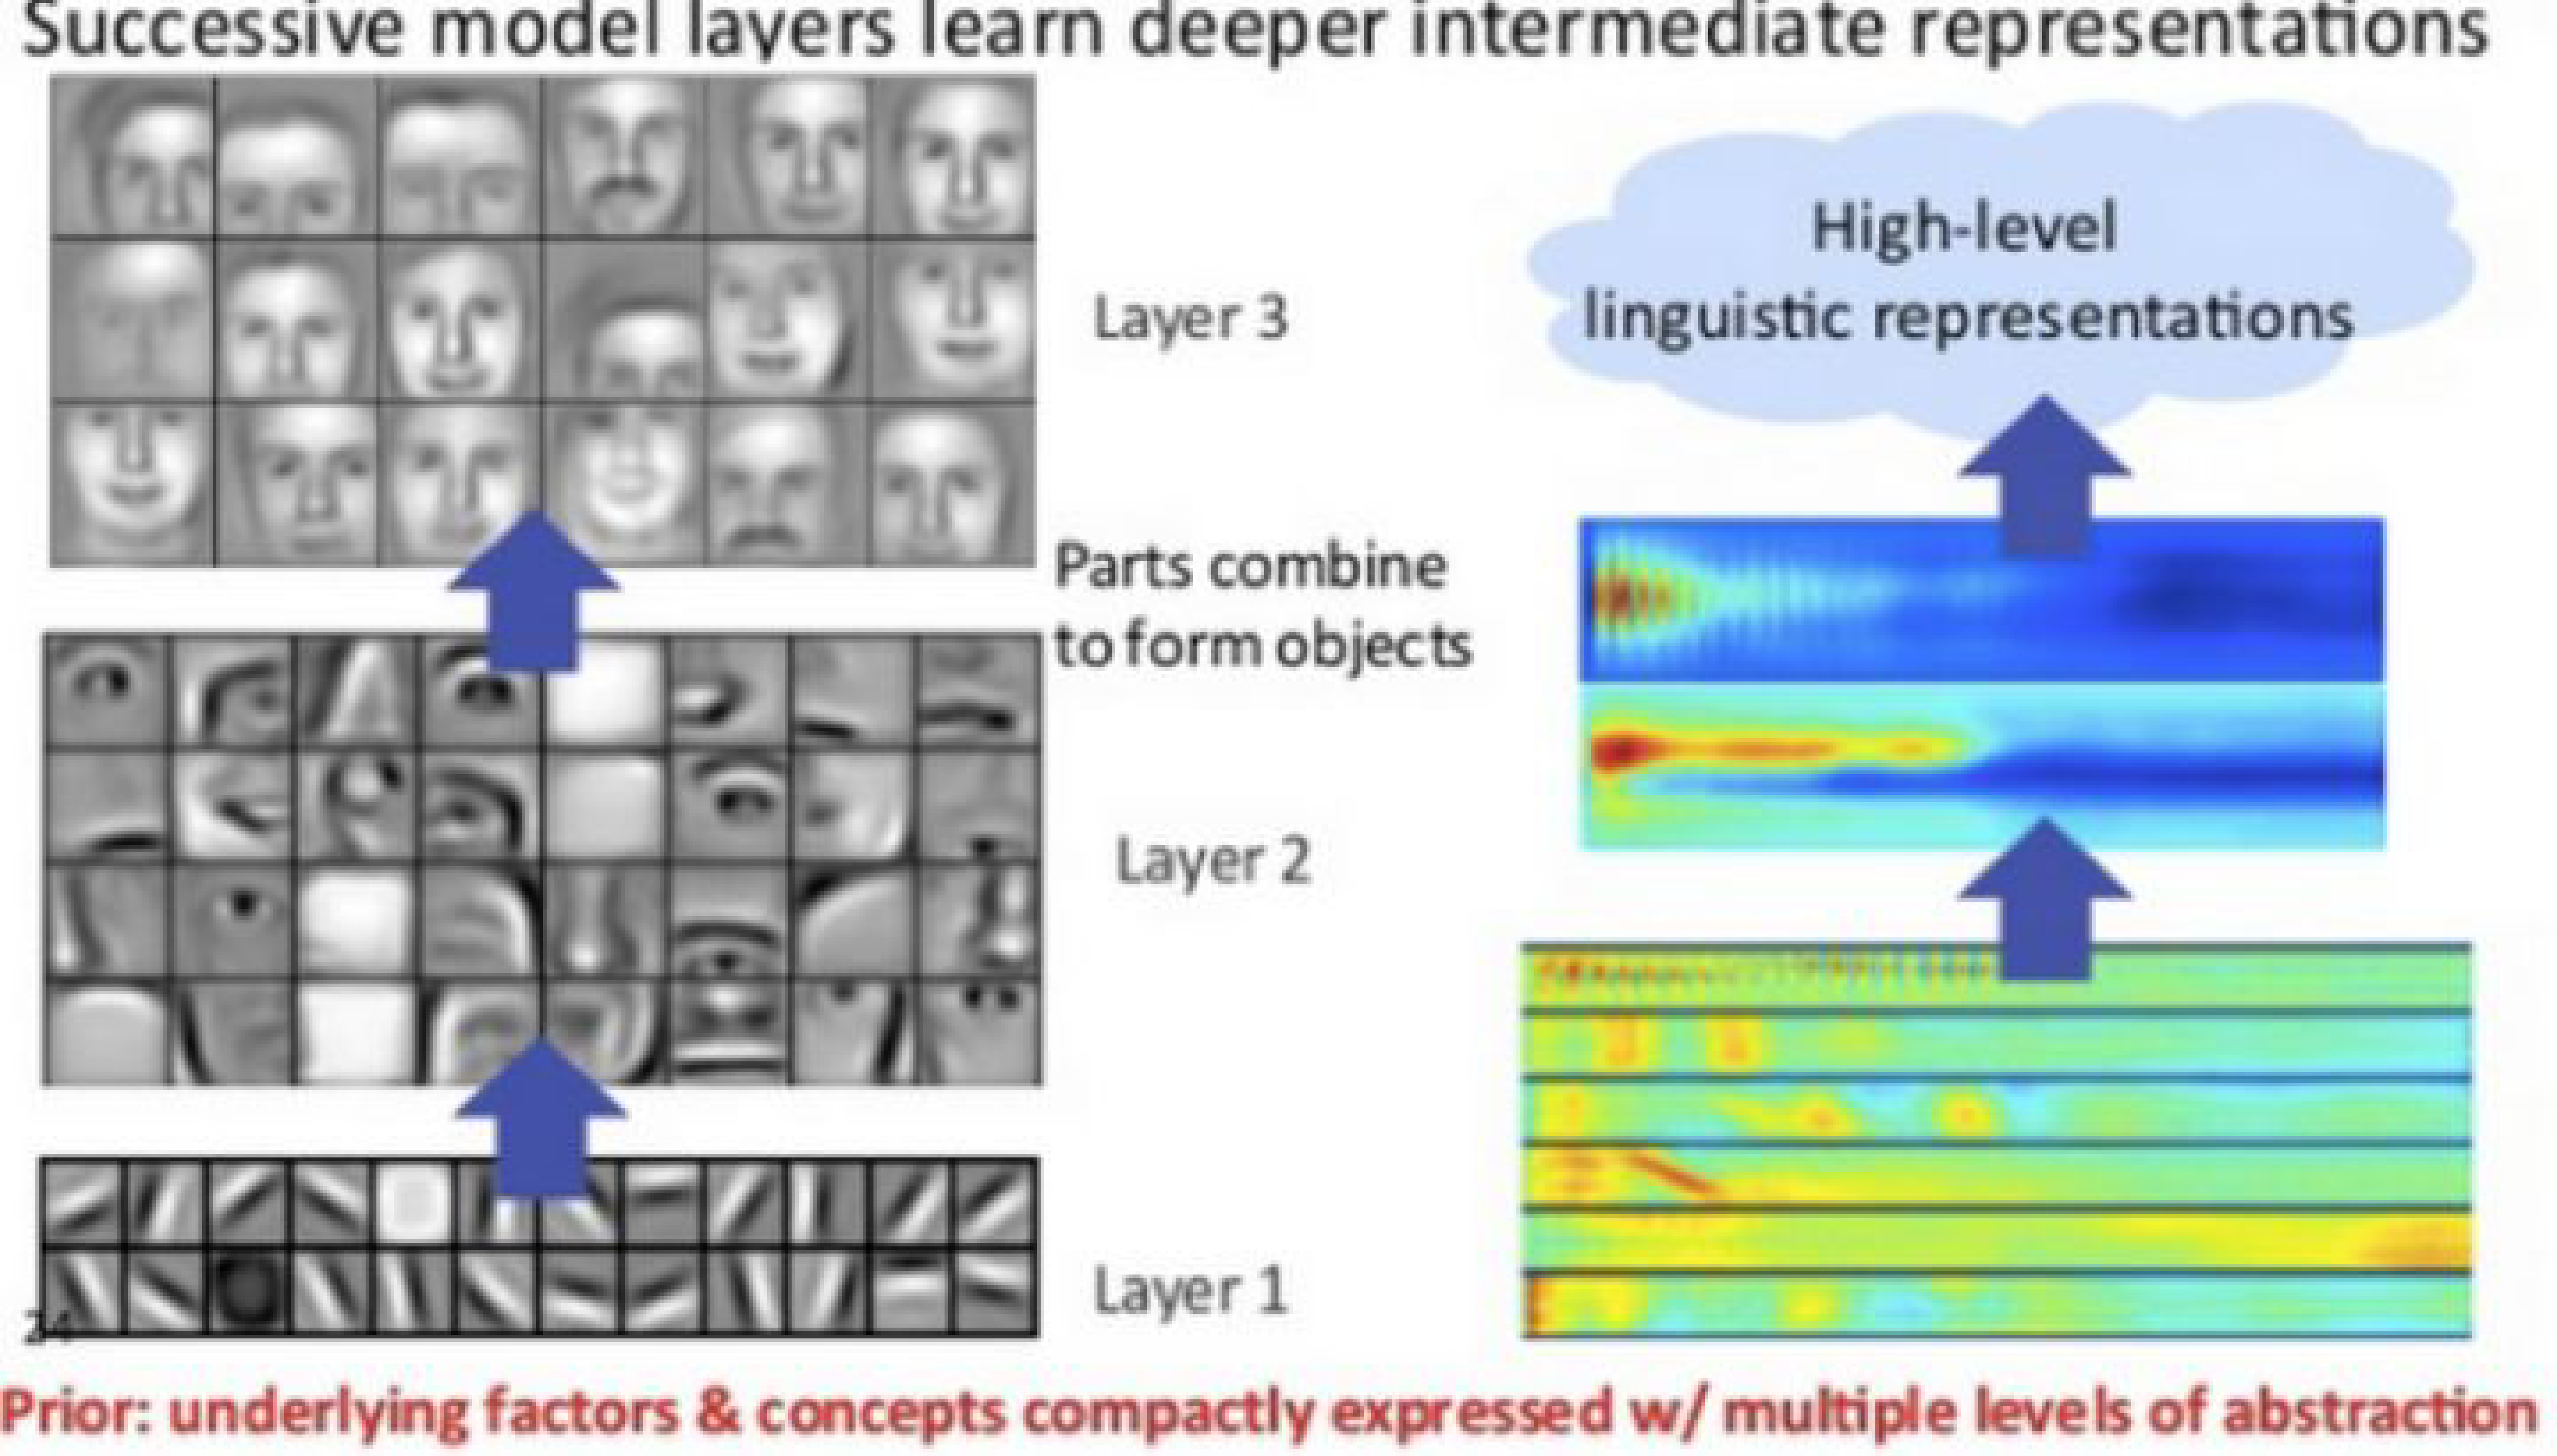
\includegraphics[scale=0.5]{./figures/fig-whydeep.pdf}
	\caption{深度神经网络进行特征提取到分类的简单示例}
	\label{fig-whydeep}
\end{figure}

这表达了一个什么事实呢?概括来说就是:前面几层都学习到的是通用的特征(general feature);随着网络层次的加深,后面的网络更偏重于学习任务特定的特征(specific feature)。这非常好理解,我们也都很好接受。那么问题来了:如何得知哪些层能够学习到general feature,哪些层能够学习到specific feature。更进一步:\textit{如果应用于迁移学习,如何决定该迁移哪些层、固定哪些层?}

这个问题对于理解神经网络以及深度迁移学习都有着非常重要的意义。

来自康奈尔大学的Jason Yosinski等人~\cite{yosinski2014transferable}率先进行了深度神经网络可迁移性的研究,将成果发表在2014年机器学习领域顶级会议NIPS上并做了口头汇报。该论文是一篇实验性质的文章(通篇没有一个公式)。其目的就是要探究上面我们提到的几个关键性问题。因此,文章的全部贡献都来自于实验及其结果。(别说为啥做实验也能发文章:都是高考,我只上了个普通一本,我高中同学就上了清华)

在ImageNet的1000类上,作者把1000类分成两份(A和B),每份500个类别。然后,分别对A和B基于Caffe训练了一个AlexNet网络。一个AlexNet网络一共有8层,除去第8层是类别相关的网络无法迁移以外,作者在1到7这7层上逐层进行finetune实验,探索网络的可迁移性。

为了更好地说明finetune的结果,作者提出了有趣的概念:AnB和BnB。

迁移A网络的前$n$层到B(AnB) vs 固定B网络的前$n$层(BnB)

简单说一下什么叫AnB:(所有实验都是针对数据B来说的)将A网络的前$n$层拿来并将它frozen,剩下的$8-n$层随机初始化,然后对B进行分类。

相应地,有BnB:把训练好的B网络的前$n$层拿来并将它frozen,剩下的$8-n$层随机初始化,然后对B进行分类。

\textbf{实验结果}

实验结果如下图(图~\ref{fig-8-2})所示:

\begin{figure}[htbp]
	\centering
	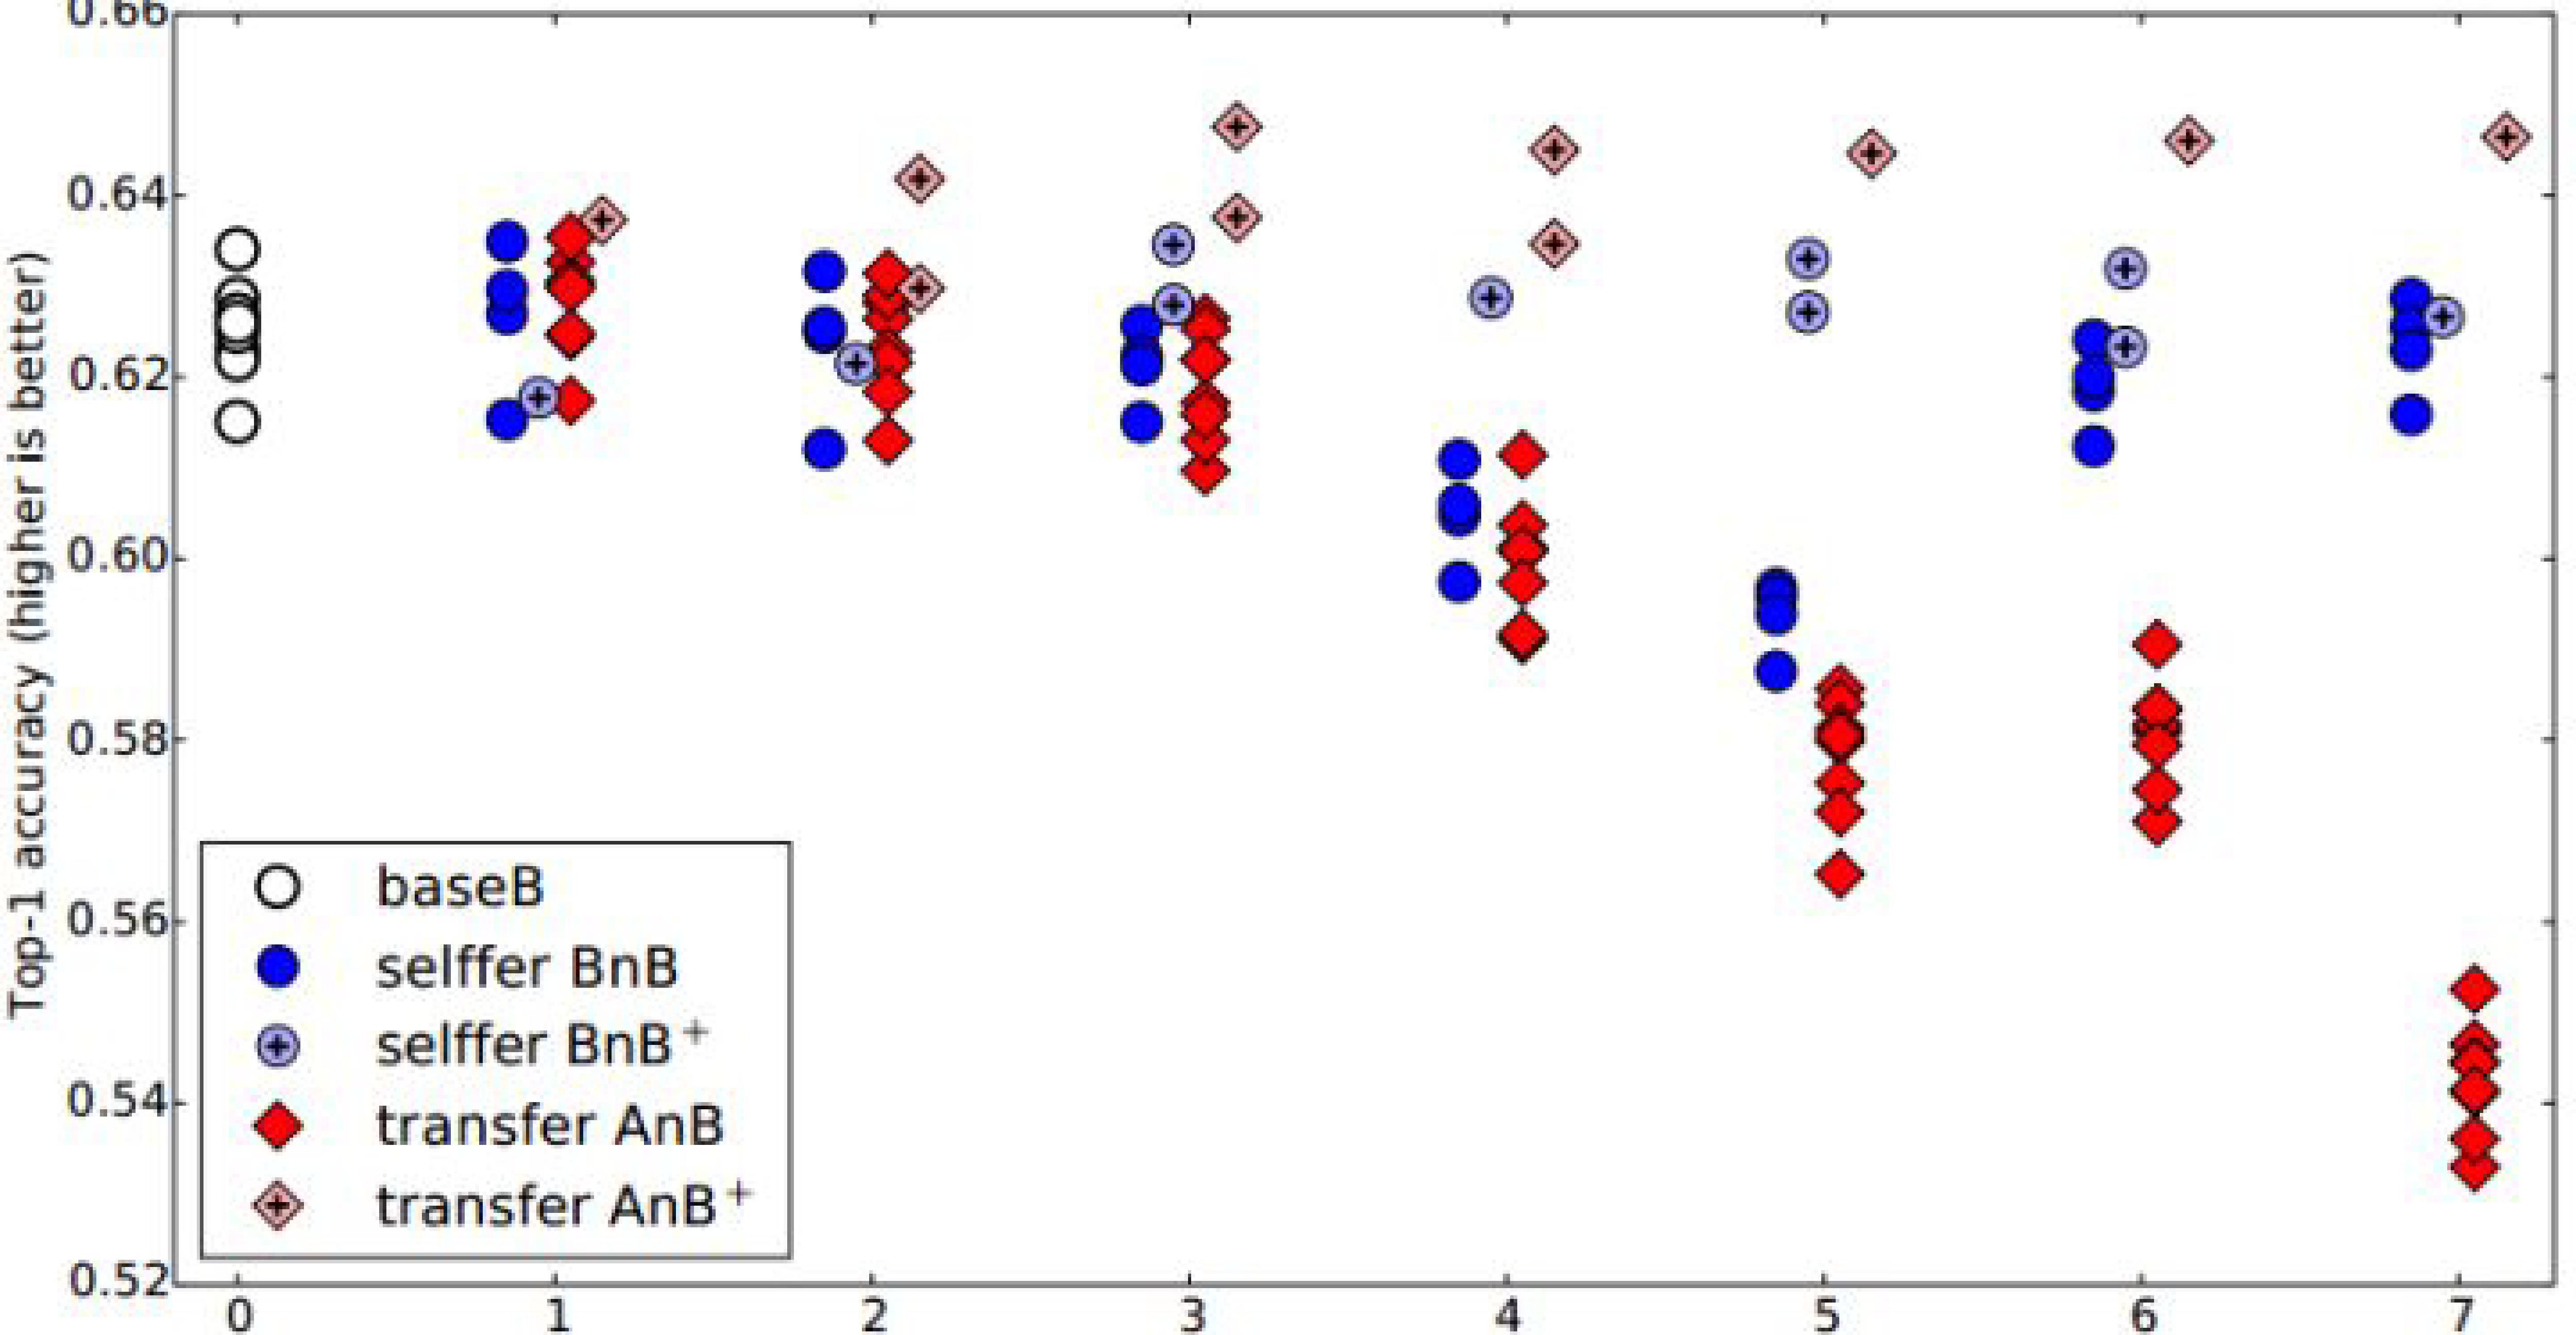
\includegraphics[scale=0.5]{figures/fig-8_1.pdf}
	\caption{深度网络迁移实验结果1}
	\label{fig-8-2}
\end{figure}

这个图说明了什么呢?我们先看蓝色的BnB和BnB+(就是BnB加上finetune)。对BnB而言,原训练好的B模型的前3层直接拿来就可以用而不会对模型精度有什么损失。到了第4和第5层,精度略有下降,不过还是可以接受。然而到了第6第第7层,精度居然奇迹般地回升了!这是为什么?原因如下:对于一开始精度下降的第4第5层来说,确实是到了这一步,feature变得越来越specific,所以下降了。那对于第6第7层为什么精度又不变了?那是因为,整个网络就8层,我们固定了第6第7层,这个网络还能学什么呢?所以很自然地,精度和原来的B网络几乎一致!

对BnB+来说,结果基本上都保持不变。说明finetune对模型结果有着很好的促进作用!

我们重点关注AnB和AnB+。对AnB来说,直接将A网络的前3层迁移到B,貌似不会有什么影响,再一次说明,网络的前3层学到的几乎都是general feature!往后,到了第4第5层的时候,精度开始下降,我们直接说:一定是feature不general了!然而,到了第6第7层,精度出现了小小的提升后又下降,这又是为什么?作者在这里提出两点:co-adaptation和feature representation。就是说,第4第5层精度下降的时候,主要是由于A和B两个数据集的差异比较大,所以会下降;到了第6第7层,由于网络几乎不迭代了,学习能力太差,此时feature学不到,所以精度下降得更厉害。

再看AnB+。加入了finetune以后,AnB+的表现对于所有的$n$几乎都非常好,甚至比baseB(最初的B)还要好一些!这说明:finetune对于深度迁移有着非常好的促进作用!

把上面的结果合并就得到了下面一张图(图~\ref{fig-8-3}):

\begin{figure}[htbp]
	\centering
	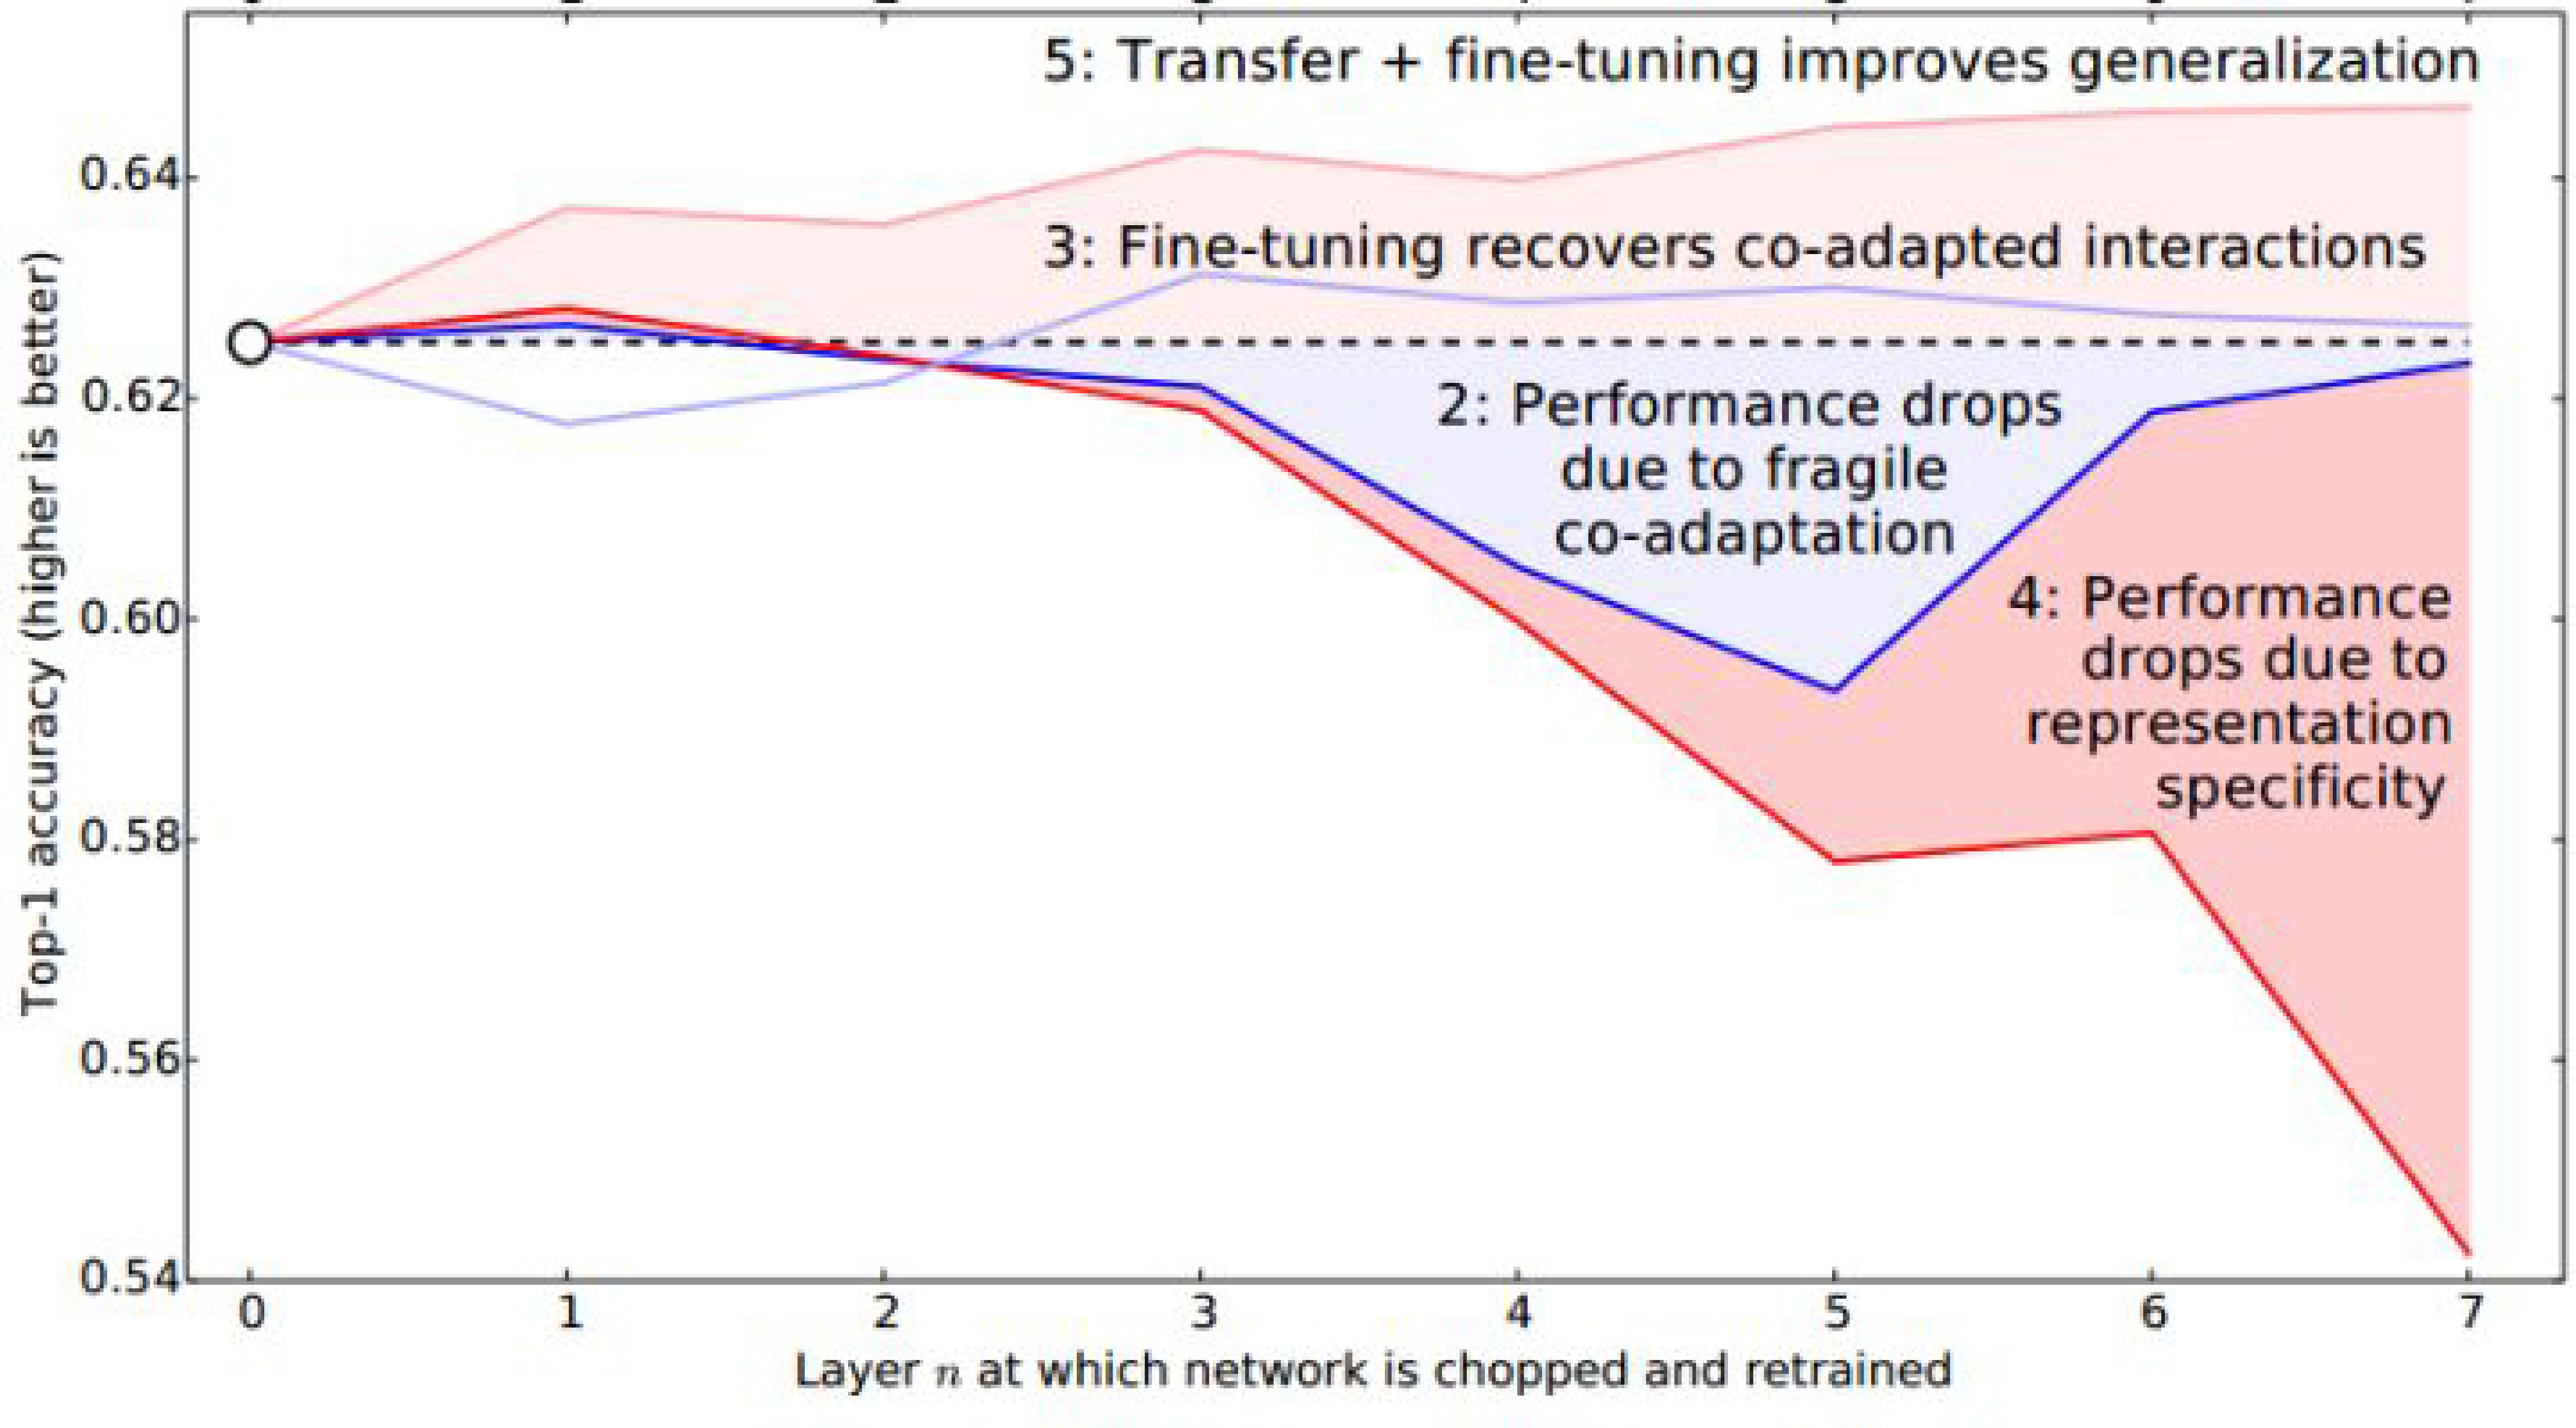
\includegraphics[scale=0.5]{figures/fig-8_2.pdf}
	\caption{深度网络迁移实验结果2}
	\label{fig-8-3}
\end{figure}

至此,AnB和BnB基本完成。作者又想,是不是我分A和B数据的时候,里面存在一些比较相似的类使结果好了?比如说A里有猫,B里有狮子,所以结果会好?为了排除这些影响,作者又分了一下数据集,这次使得A和B里几乎没有相似的类别。在这个条件下再做AnB,与原来精度比较(0\%为基准)得到了下图(图~\ref{fig-8-4}):

\begin{figure}[htbp]
	\centering
	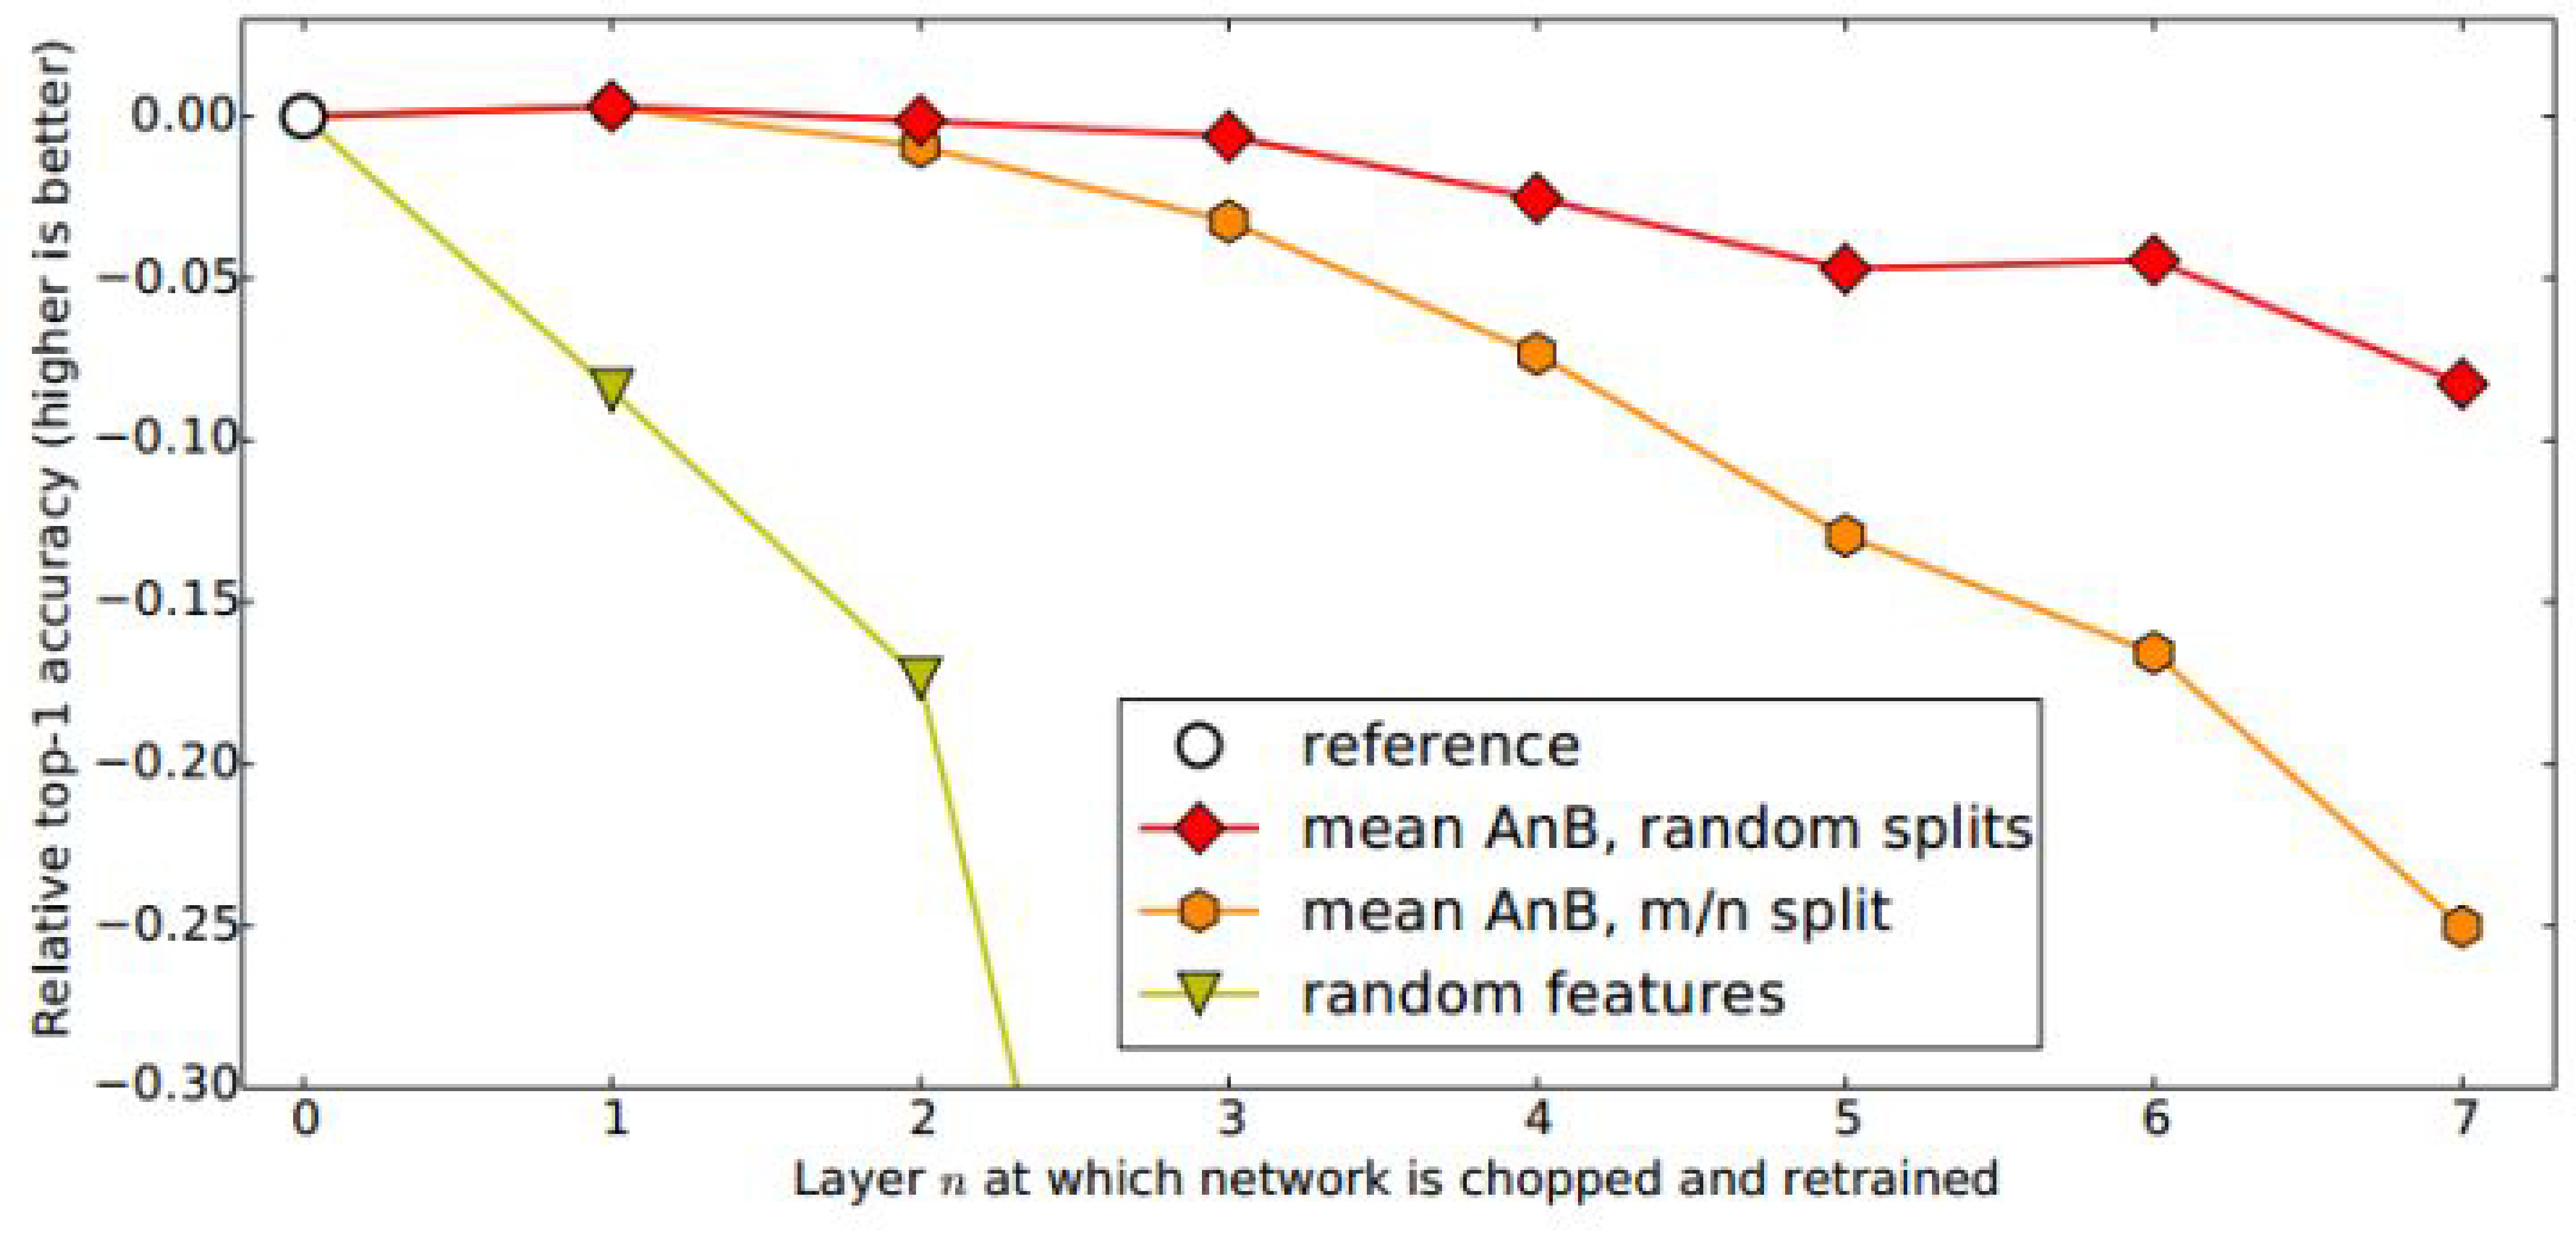
\includegraphics[scale=0.5]{./figures/fig-8_3.pdf}
	\caption{深度网络迁移实验结果3}
	\label{fig-8-4}
\end{figure}

这个图说明了什么呢?简单:随着可迁移层数的增加,模型性能下降。但是,前3层仍然还是可以迁移的!同时,与随机初始化所有权重比较,迁移学习的精度是很高的!

\textbf{结论}

虽然该论文并没有提出一个创新方法,但是通过实验得到了以下几个结论,对以后的深度学习和深度迁移学习都有着非常高的指导意义:

\begin{itemize}
	\item 神经网络的前3层基本都是general feature,进行迁移的效果会比较好;
	\item 深度迁移网络中加入fine-tune,效果会提升比较大,可能会比原网络效果还好;
	\item Fine-tune可以比较好地克服数据之间的差异性;
	\item 深度迁移网络要比随机初始化权重效果好;
	\item 网络层数的迁移可以加速网络的学习和优化。
\end{itemize}

\subsection{最简单的深度迁移:finetune}

深度网络的finetune也许是最简单的深度网络迁移方法。\textbf{Finetune},也叫微调、finetuning,是深度学习中的一个重要概念。简而言之,finetune就是利用别人已经训练好的网络,针对自己的任务再进行调整。从这个意思上看,我们不难理解finetune是迁移学习的一部分。

\textbf{1. 为什么需要已经训练好的网络?}

在实际的应用中,我们通常不会针对一个新任务,就去从头开始训练一个神经网络。这样的操作显然是非常耗时的。尤其是,我们的训练数据不可能像ImageNet那么大,可以训练出泛化能力足够强的深度神经网络。即使有如此之多的训练数据,我们从头开始训练,其代价也是不可承受的。

那么怎么办呢?迁移学习告诉我们,利用之前已经训练好的模型,将它很好地迁移到自己的任务上即可。

\textbf{2. 为什么需要finetune?}

因为别人训练好的模型,可能\textit{并不是完全适用}于我们自己的任务。可能别人的训练数据和我们的数据之间不服从同一个分布;可能别人的网络能做比我们的任务更多的事情;可能别人的网络比较复杂,我们的任务比较简单。

举一个例子来说,假如我们想训练一个猫狗图像二分类的神经网络,那么很有参考价值的就是在CIFAR-100上训练好的神经网络。但是CIFAR-100有100个类别,我们只需要2个类别。此时,就需要针对我们自己的任务,固定原始网络的相关层,修改网络的输出层,以使结果更符合我们的需要。

图~\ref{fig-deep-finetune}展示了一个简单的finetune过程。从图中我们可以看到,我们采用的预训练好的网络非常复杂,如果直接拿来从头开始训练,则时间成本会非常高昂。我们可以将此网络进行改造,固定前面若干层的参数,只针对我们的任务,微调后面若干层。这样,网络训练速度会极大地加快,而且对提高我们任务的表现也具有很大的促进作用。

\begin{figure}[htbp]
	\centering
	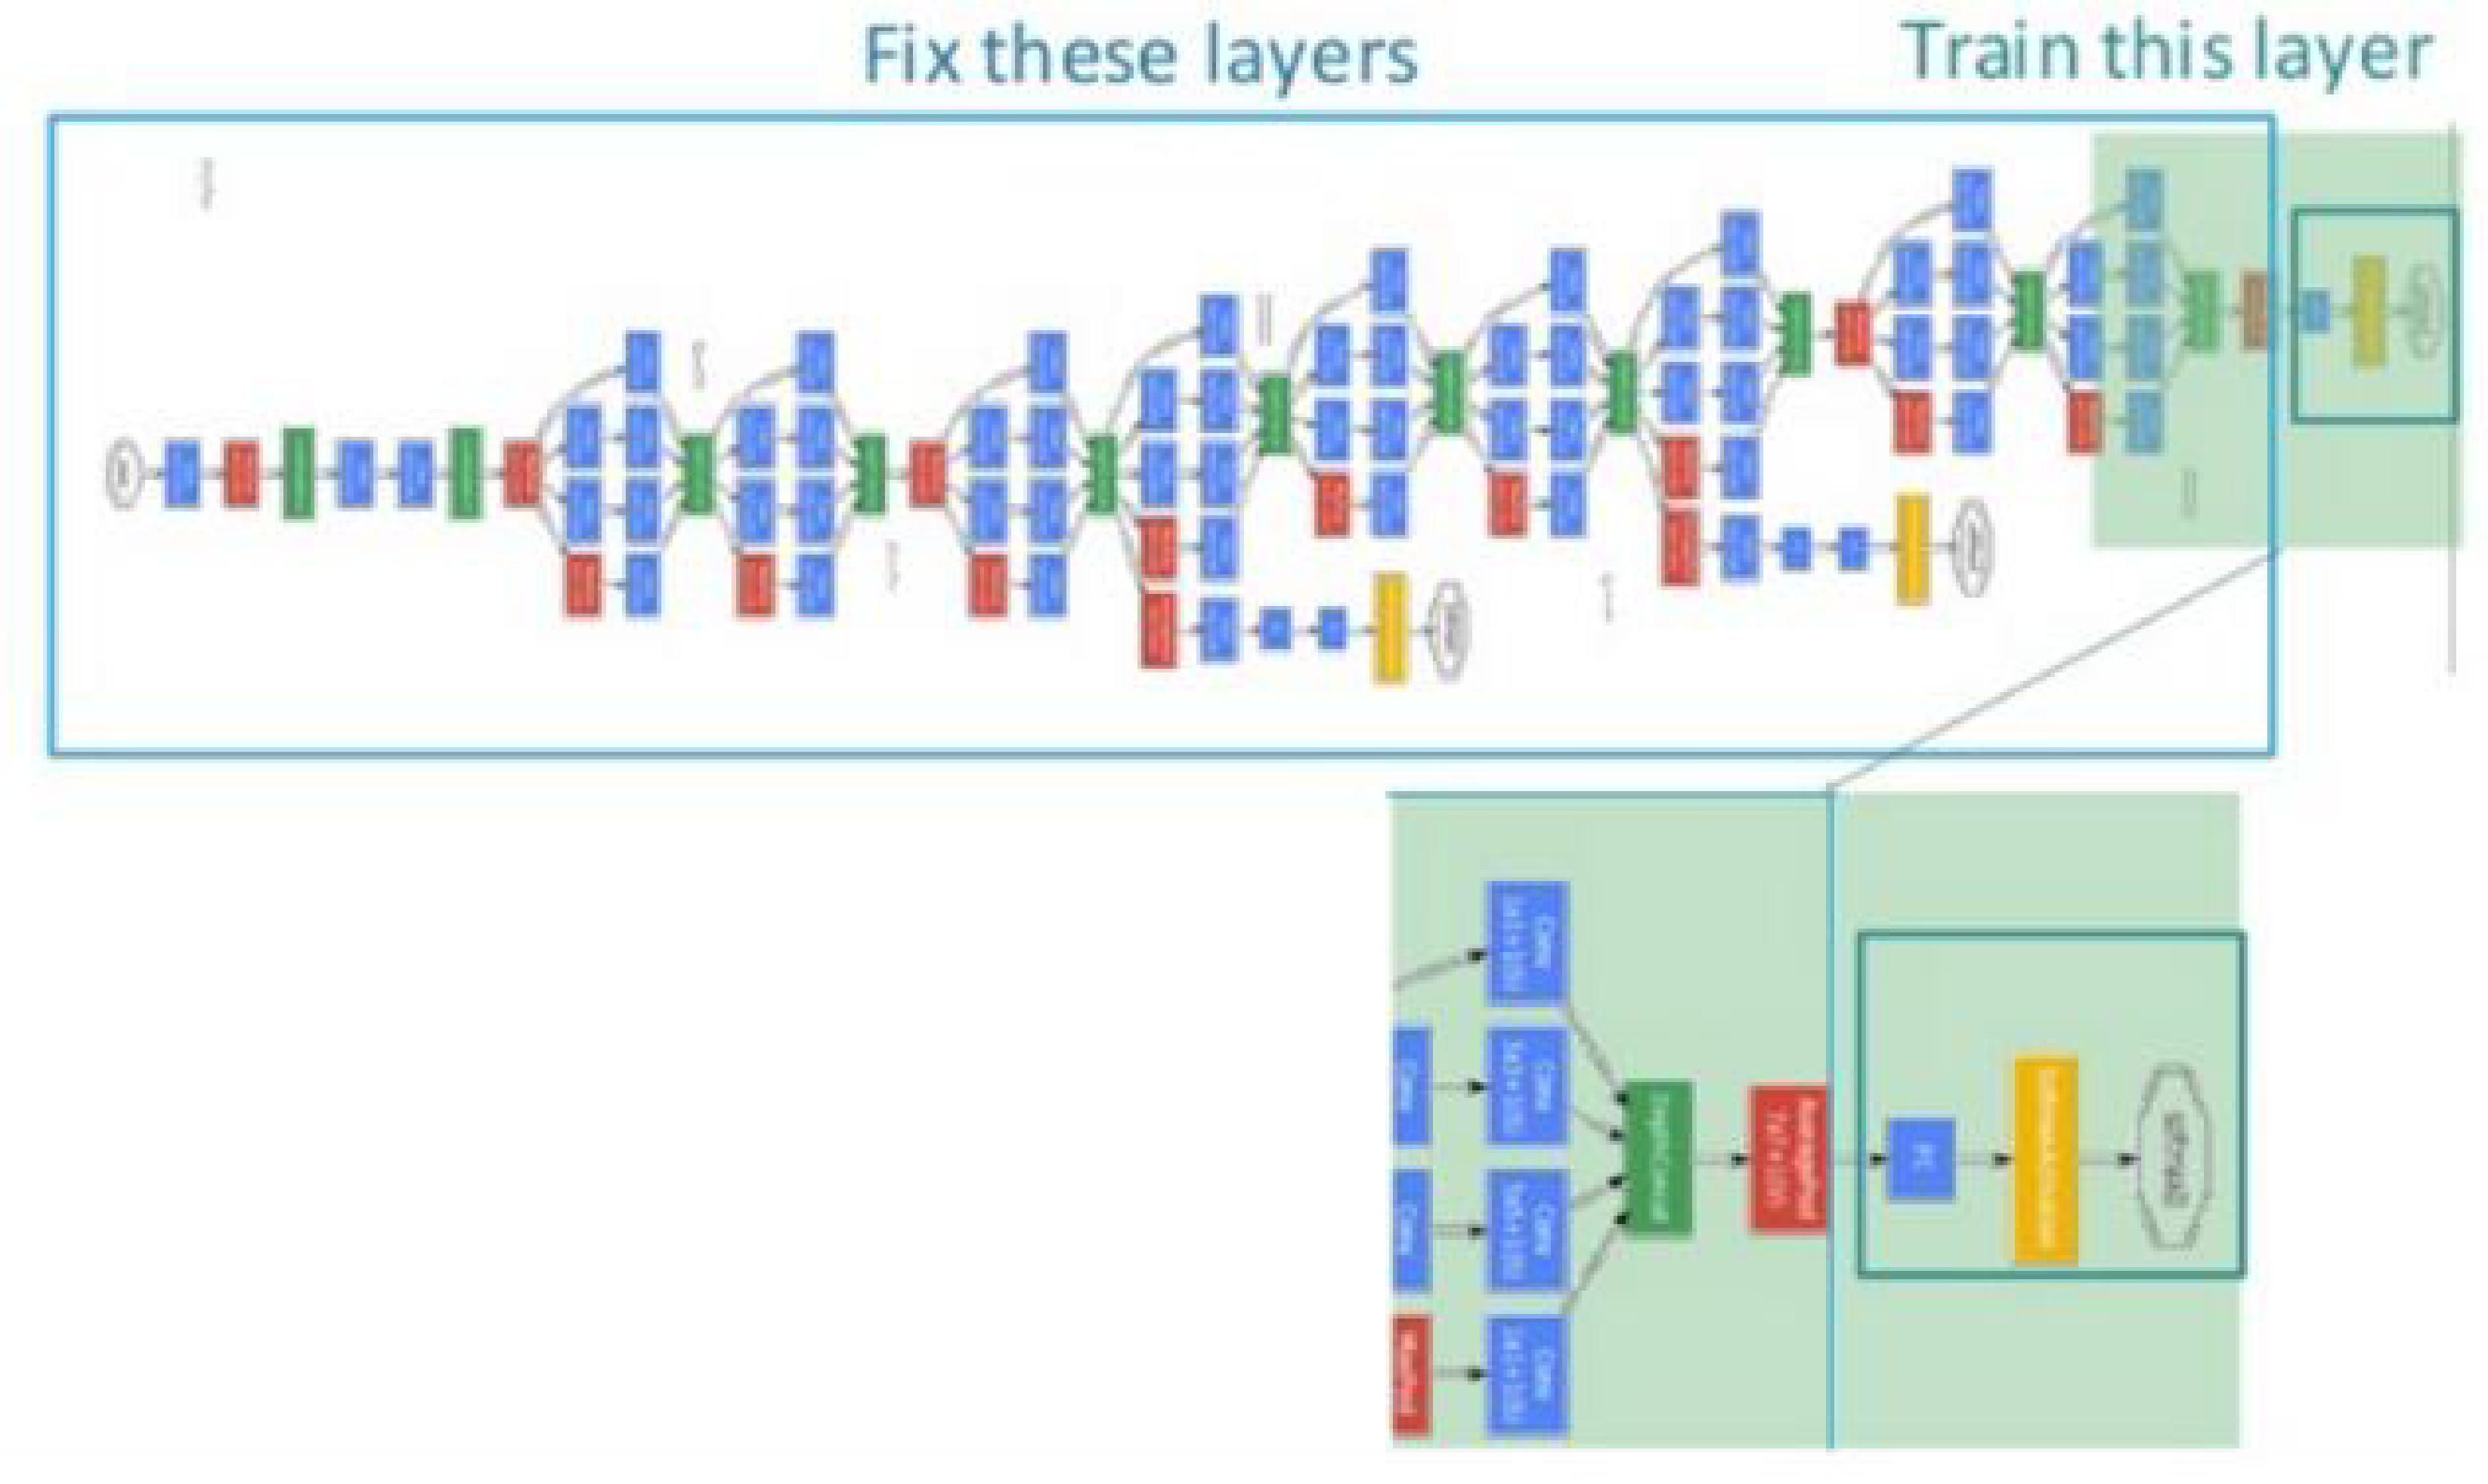
\includegraphics[scale=0.6]{./figures/fig-deep-finetune.pdf}
	\caption{一个简单的finetune示意图}
	\label{fig-deep-finetune}
\end{figure}

\textbf{3. Finetune的优势}

Finetune的优势是显然的,包括:

\begin{itemize}
	\item 不需要针对新任务从头开始训练网络,节省了时间成本;
	\item 预训练好的模型通常都是在大数据集上进行的,无形中扩充了我们的训练数据,使得模型更鲁棒、泛化能力更好;
	\item Finetune实现简单,使得我们只关注自己的任务即可。
\end{itemize}

\textbf{4. Finetune的扩展}

在实际应用中,通常几乎没有人会针对自己的新任务从头开始训练一个神经网络。Finetune是一个理想的选择。

Finetune并不只是针对深度神经网络有促进作用,对传统的非深度学习也有很好的效果。例如,finetune对传统的人工提取特征方法就进行了很好的替代。我们可以使用深度网络对原始数据进行训练,依赖网络提取出更丰富更有表现力的特征。然后,将这些特征作为传统机器学习方法的输入。这样的好处是显然的:\textit{既避免了繁复的手工特征提取,又能自动地提取出更有表现力的特征。}

比如,图像领域的研究,一直是以SIFT、SURF等传统特征为依据的,直到2014年,伯克利的研究人员提出了DeCAF特征提取方法~\cite{donahue2014decaf},直接使用深度卷积神经网络进行特征提取。实验结果表明,该特征提取方法对比传统的图像特征,在精度上有着无可匹敌的优势。另外,也有研究人员用卷积神经网络提取的特征作为SVM分类器的输入~\cite{razavian2014cnn},显著提升了图像分类的精度。

\subsection{深度网络自适应}

\subsubsection{基本思路}

深度网络的finetune可以帮助我们节省训练时间,提高学习精度。但是finetune有它的先天不足:它无法处理训练数据和测试数据分布不同的情况。而这一现象在实际应用中比比皆是。因为finetune的基本假设也是训练数据和测试数据服从相同的数据分布。这在迁移学习中也是不成立的。因此,我们需要更进一步,针对深度网络开发出更好的方法使之更好地完成迁移学习任务。

以我们之前介绍过的数据分布自适应方法为参考,许多深度学习方法~\cite{tzeng2014deep,long2015learning}都开发出了\textit{自适应层}(Adaptation Layer)来完成源域和目标域数据的自适应。自适应能够使得源域和目标域的数据分布更加接近,从而使得网络的效果更好。

从上述的分析我们可以得出,深度网络的自适应主要完成两部分的工作:

一是哪些层可以自适应,这决定了网络的学习程度;

二是采用什么样的自适应方法(度量准则),这决定了网络的泛化能力。

深度网络中最重要的是网络损失的定义。绝大多数深度迁移学习方法都采用了以下的损失定义方式:

\begin{equation}
	\ell = \ell_c(\mathcal{D}_s,\mathbf{y}_s) + \lambda \ell_A(\mathcal{D}_s,\mathcal{D}_t)
\end{equation}

其中,$\ell$表示网络的最终损失,$\ell_c(\mathcal{D}_s,\mathbf{y}_s)$表示网络在有标注的数据(大部分是源域)上的常规分类损失(这与普通的深度网络完全一致),$\ell_A(\mathcal{D}_s,\mathcal{D}_t)$表示网络的自适应损失。最后一部分是传统的深度网络所不具有的、迁移学习所独有的。此部分的表达与我们先前讨论过的源域和目标域的分布差异,在道理上是相同的。式中的$\lambda$是权衡两部分的权重参数。

上述的分析指导我们设计深度迁移网络的基本准则:决定自适应层,然后在这些层加入自适应度量,最后对网络进行finetune。

\subsubsection{核心方法}

前期的研究者在2014年环太平洋人工智能大会(PRICAI)上提出了一个叫做DaNN(Domain Adaptive Neural Network)的神经网络~\cite{ghifary2014domain}。DaNN的结构异常简单,它仅由两层神经元组成:特征层和分类器层。作者的创新工作在于,在特征层后加入了一项MMD适配层,用来计算源域和目标域的距离,并将其加入网络的损失中进行训练。

但是,由于网络太浅,表征能力有限,故无法很有效地解决domain adaptation问题。因此,后续的研究者大多数都基于其思想进行扩充,如将浅层网络改为更深层的AlexNet、ResNet、VGG等;如将MMD换为多核的MMD等。

\textbf{1. 第一个方法:DDC}

加州大学伯克利分校的Tzeng等人~\cite{tzeng2014deep}首先提出了一个DDC方法(Deep Domain Confusion)解决深度网络的自适应问题。DDC遵循了我们上述讨论过的基本思路,采用了在ImageNet数据集上训练好的AlexNet网络~\cite{krizhevsky2012imagenet}进行自适应学习。

图~\ref{fig-deep-ddc}是DDC方法的示意。DDC固定了AlexNet的前7层,在第8层(分类器前一层)上加入了自适应的度量。自适应度量方法采用了被广泛使用的MMD准则。DDC方法的损失函数表示为:

\begin{equation}
	\label{eq-deep-ddc}
	\ell = \ell_c(\mathcal{D}_s,\mathbf{y}_s) + \lambda MMD^2(\mathcal{D}_s,\mathcal{D}_t)
\end{equation}

\begin{figure}[htbp]
	\centering
	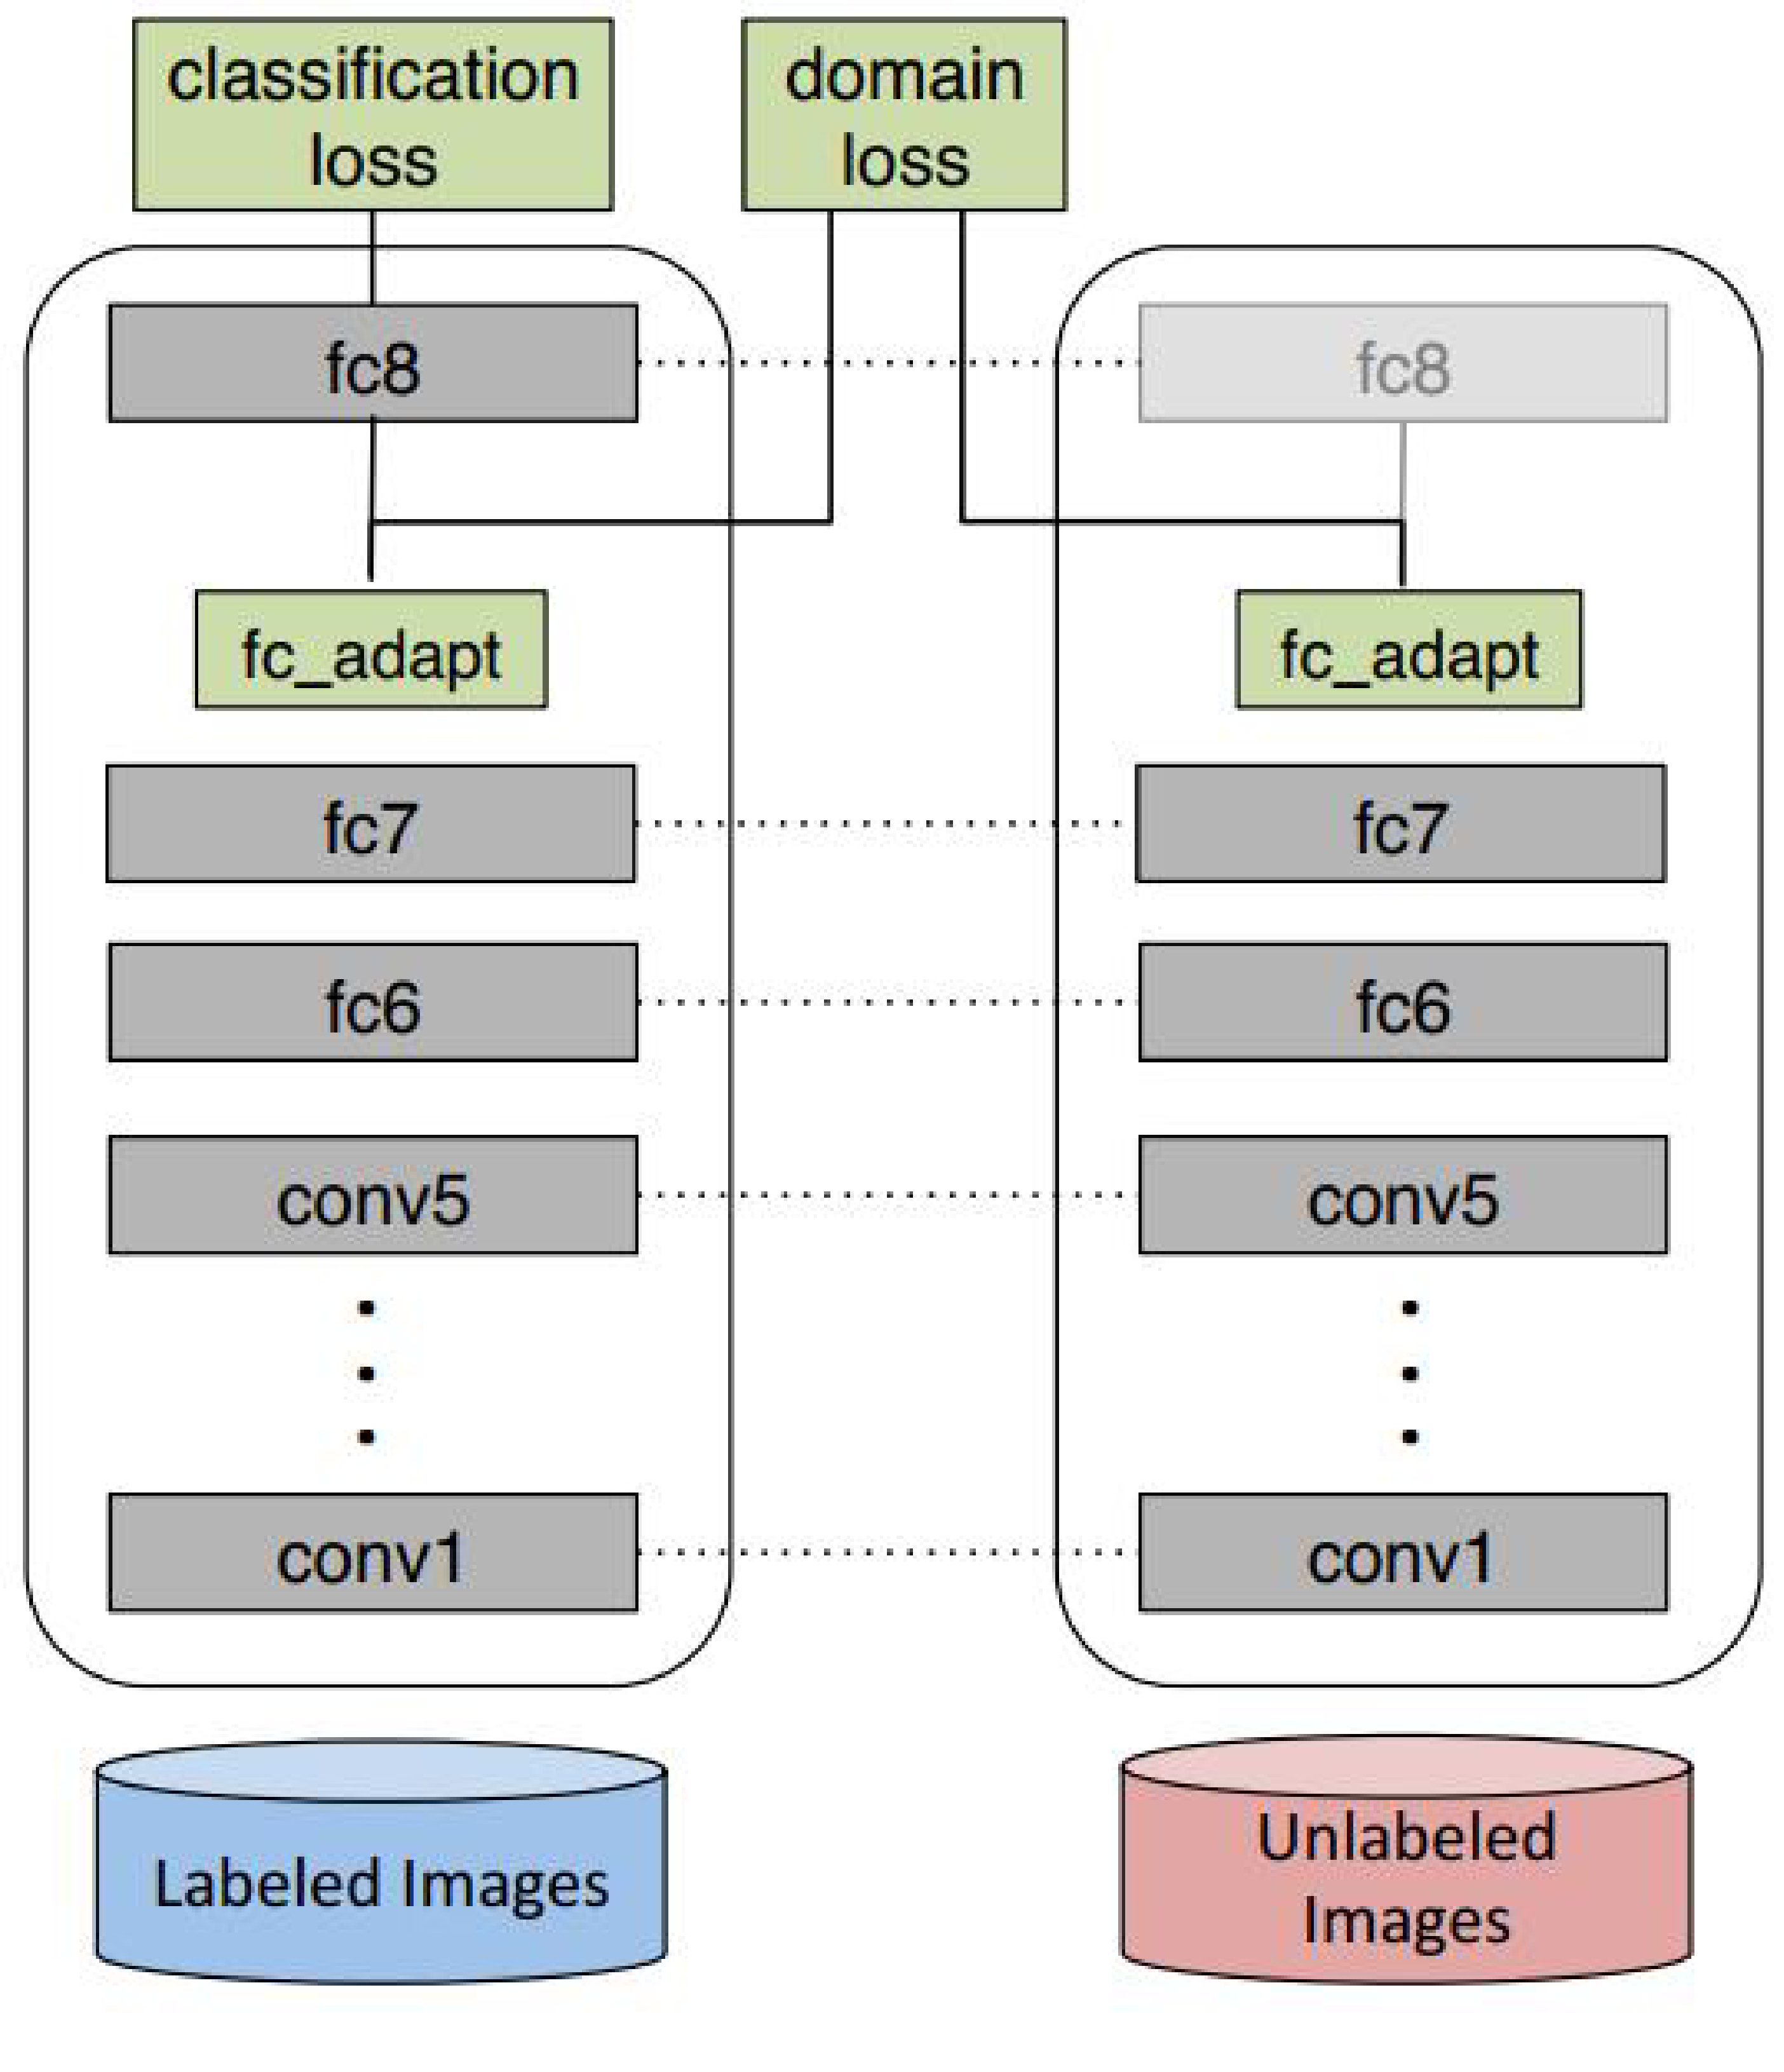
\includegraphics[scale=0.6]{./figures/fig-deep-ddc.pdf}
	\caption{DDC方法示意图}
	\label{fig-deep-ddc}
\end{figure}

\textbf{为什么选择了倒数第二层?} DDC方法的作者在文章中提到,他们经过了多次实验,在不同的层进行了尝试,最终得出结论,在分类器前一层加入自适应可以达到最好的效果。

这也是与我们的认知相符合的。通常来说,分类器前一层即特征,在特征上加入自适应,也正是迁移学习要完成的工作。

\textbf{2. DAN}

来自清华大学的龙明盛等人在2015年发表在机器学习顶级会议ICML上的DAN方法(Deep Adaptation Networks)~\cite{long2015learning}对DDC方法进行了几个方面的扩展。首先,有别于DDC方法只加入一个自适应层,DAN方法同时加入了三个自适应层(分类器前三层)。其次,DAN方法采用了表征能力更好的多核MMD度量(MK-MMD)~\cite{gretton2012optimal}代替了DDC方法中的单一核MMD。然后,DAN方法将多核MMD的参数学习融入到深度网络的训练中,不增加网络的额外训练时间。DAN方法在多个任务上都取得了比DDC更好的分类效果。

为什么是适配3层?原来的DDC方法只是适配了一层,现在DAN也基于AlexNet网络,适配最后三层(第6第7第8层)。为什么是这三层?因为在Jason的文章~\cite{yosinski2014transferable}中已经说了,网络的迁移能力在这三层开始就会特别地task-specific,所以要着重适配这三层。至于别的网络(比如GoogLeNet、VGG)等是不是这三层就需要通过自己的实验来推测。DAN只关注使用AlexNet。

MK-MMD的多核表示形式为

\begin{equation}
	\mathcal{K} \triangleq \left\{k= \sum_{u=1}^{m}\beta_u k_u : \beta_u \ge 0, \forall u \right\}
\end{equation}

DAN的优化目标也由两部分组成:损失函数和自适应损失。损失函数这个好理解,基本上所有的机器学习方法都会定义一个损失函数,它来度量预测值和真实值的差异。分布距离就是我们上面提到的MK-MMD距离。于是,DAN的优化目标就是

\begin{equation}
	\label{eq-deep-dan}
	\min_\Theta \frac{1}{n_a} \sum_{i=1}^{n_a} J(\theta(\mathbf{x}^a_i),y^a_i) + \lambda \sum_{l=l_1}^{l_2}d^2_k(\mathcal{D}^l_s,\mathcal{D}^l_t)
\end{equation}

这个式子中,$\Theta$表示网络的所有权重和bias参数,是用来学习的目标。其中$l_1,l_2$分别是6和8,表示网络适配是从第6层到第8层,前面的不进行适配。$\mathbf{x}_a,n_a$表示源域和目标域中所有有标注的数据的集合。$J(\cdot)$就定义了一个损失函数,在深度网络中一般都是cross-entropy。DAN的网络结构如下图所示。

\begin{figure}[htbp]
	\centering
	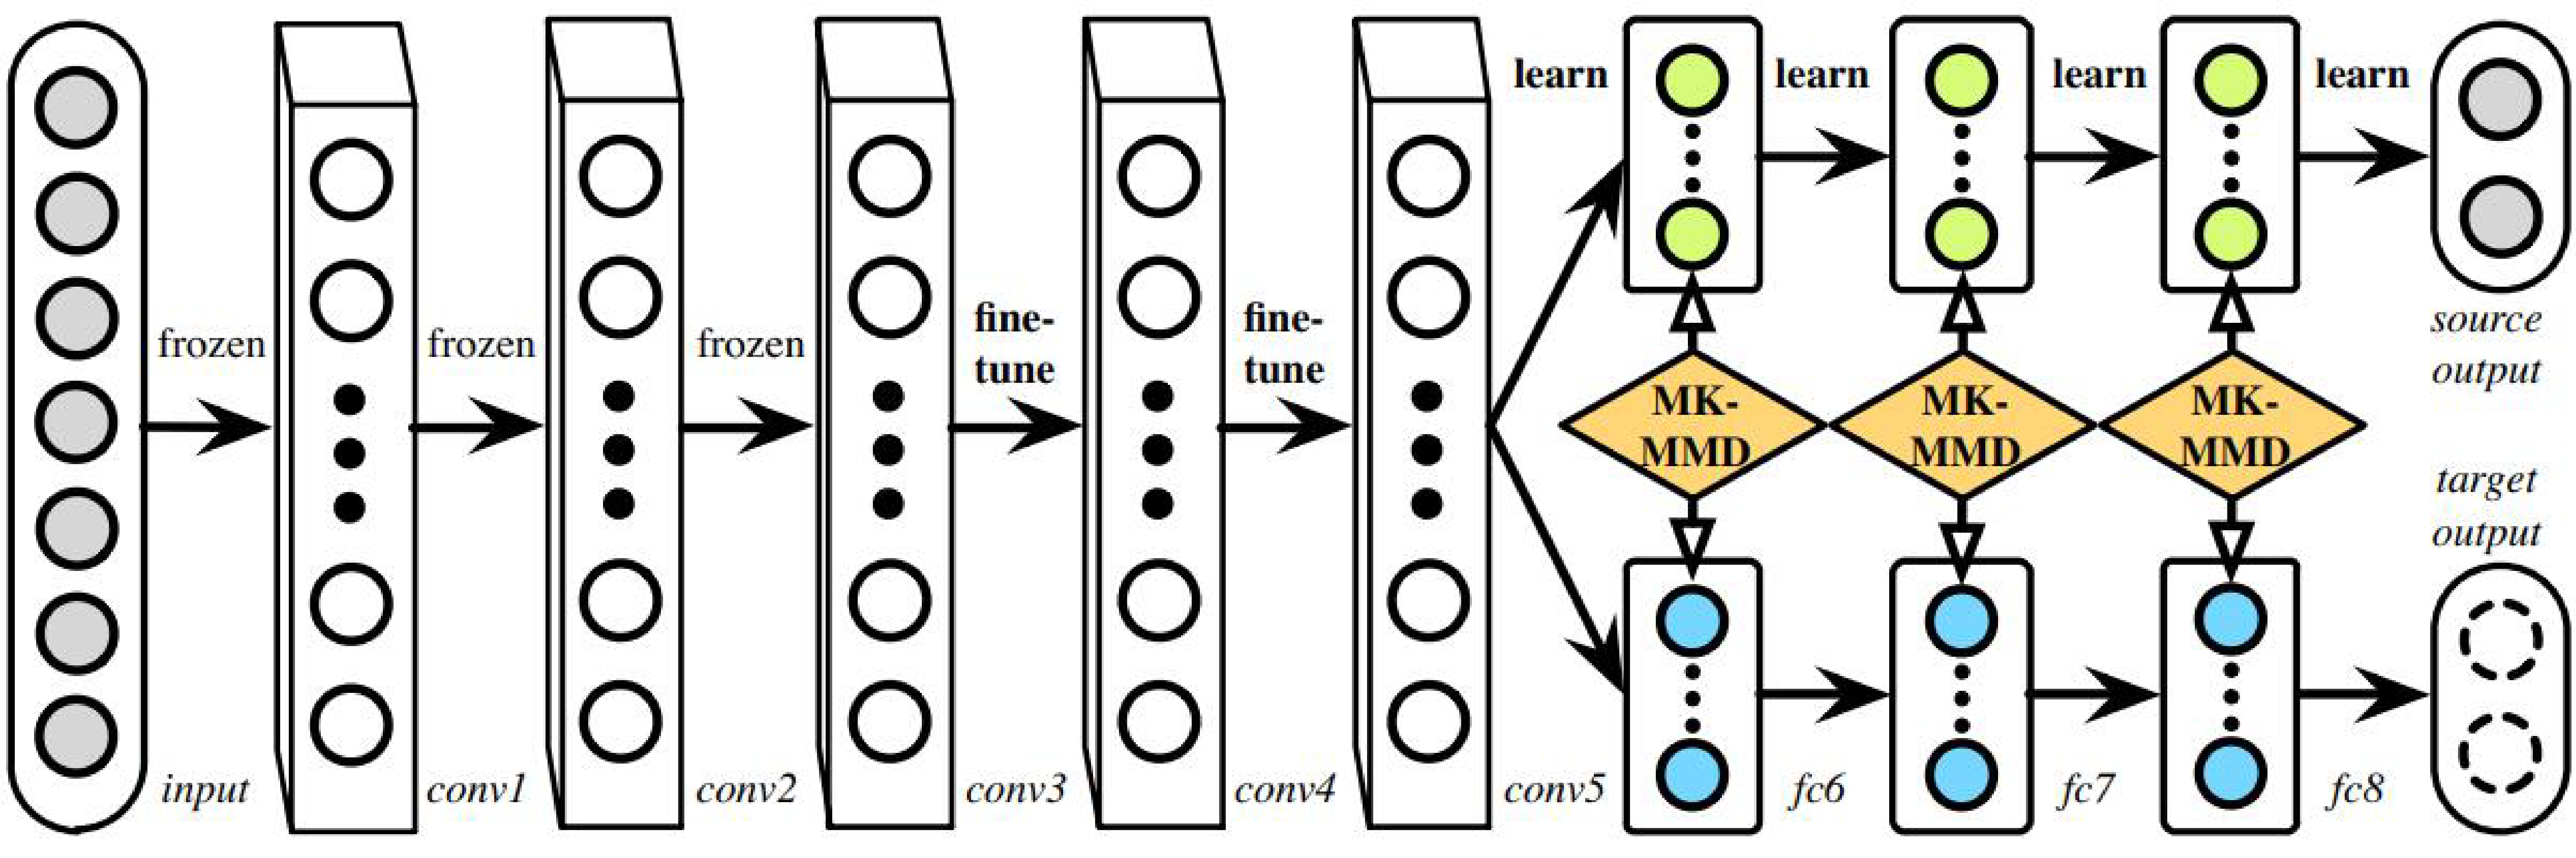
\includegraphics[scale=0.45]{./figures/fig-deep-dan.pdf}
	\caption{DAN方法示意图}
	\label{fig-deep-dan}
\end{figure}

\textbf{学习策略}

DAN的学习一共分为两大类参数:学习网络参数$\Theta$和MMD的$\beta$。

对$\Theta$的学习依赖于MK-MMD距离的计算。通过kernel trick(类比以前的MMD变换)我们总是可以把MK-MMD展开成一堆内积的形式。然而,数据之间两两计算内积是非常复杂的,时间复杂度为$O(n^2)$,这个在深度学习中的开销非常之大。怎么办?作者在这里采用了Gretton在文章~\cite{gretton2012optimal}提出的对MK-MMD的无偏估计:$d^2_k(p,q)=\frac{2}{n_s}\sum_{i=1}^{n_s/2}g_k(\mathbf{z}_i)$,其中的$\mathbf{z}_i$是一个四元组:$\mathbf{z}_i \triangleq (\mathbf{x}^s_{2i-1},\mathbf{x}^s_{2i},\mathbf{x}^t_{2i-1},\mathbf{x}^t_{2i})$。将kernel作用到$\mathbf{z}_i$上以后,变成$g_k(\mathbf{z}_i) \triangleq k(\mathbf{x}^s_{2i-1},\mathbf{x}^s_{2i})+k(\mathbf{x}^t_{2i-1},\mathbf{x}^t_{2i})-k(\mathbf{x}^s_{2i-1},\mathbf{x}^t_{2i})-k(\mathbf{x}^s_{2i},\mathbf{x}^t_{2i-1})$。

上面这些变换看着很复杂。简单来说,它就是只计算了连续的一对数据的距离,再乘以2.这样就可以把时间复杂度降低到$O(n)$!至于具体的理论,可以去参考Gretton的论文,这里就不说了。

在具体进行SGD的时候,我们需要对所有的参数求导:对$\Theta$求导。在实际用multiple-kernel的时候,作者用的是多个高斯核。

学习$\beta$主要是为了确定多个kernel的权重。学习的时候,目标是:确保每个kernel生成的MMD距离的方差最小。也就是

\begin{equation}
	\max_{k \in \mathcal{K}} d^2_k(\mathcal{D}^l_s,\mathcal{D}^l_t) \sigma^{-2}_k
\end{equation}

这里的$\sigma^{-2}_k=E[g^2_k(\mathbf{z})]-[E(g_k(\mathbf{z}))]^2$是估计方差。实际求解的时候问题可以被规约成一个二次规划问题求解,具体可以参照文章。

\textbf{3. 同时迁移领域和任务}

DDC的作者Tzeng在2015年扩展了DDC方法,提出了领域和任务同时迁移的方法~\cite{tzeng2015simultaneous}。作者提出网络要进行两部分的迁移:

一是domain transfer,就是适配分布,特别地是指适配marginal distribution,但是没有考虑类别信息。如何做domain transfer:在传统深度网路的loss上,再加另一个confusion loss,作为classifier能否将两个domain进行分开的loss。两个loss一起计算,就是domain transfer。

二是task transfer,就是利用class之间的相似度,其实特指的是conditional distribution。类别之间有相似度,要利用上。类别之间的相似度:比如一个杯子与瓶子更相似,而与键盘不相似。文章的原话:it does not necessarily align the classes in the target with those in the source. Thus, we also explicity transfer the similarity structure amongst categories.

现有的深度迁移学习方法通常都只是考虑domain transfer,\textit{而没有考虑到类别之间的信息}。如何把domain和task transfer结合起来,是一个问题。

文章针对的情况是:target的部分class有少量label,剩下的class无label。

作者提出的方法名字叫做joint CNN architecture for domain and task transfer。最大的创新点是:现有的方法都是domain classifier加上一个domain confusion,就是适配。作者提出这些是不够的,因为忽略了类别之间的联系,所以提出了还要再加一个soft label loss。意思就是在source和target进行适配的时候,也要根据source的类别分布情况来进行调整target的。其实本意和JDA差不多。

相应地,文章的方法就是把这两个loss结合到一个新的CNN网络上,这个CNN是用AlexNet的结构修改成的。总的loss可以表示成几部分的和:

\begin{equation}
\begin{split}
L(x_S,y_S,x_T,y_T,\theta_D;\theta_{repr},\theta_C)=&L_C(x_S,y_S,x_T,y_T;\theta_{repr},\theta_C)\\
&+\lambda L_{conf}(x_S,x_T,\theta_D;\theta_{repr})+v L_{soft}(x_T,y_T;\theta_{repr},\theta_C)
\end{split}
\end{equation}

Loss由三部分组成:第一部分是普通训练的loss,对应于经验风险最小化,所以作用到了所有有label的数据 $x_S,y_S,x_T,y_T$上;第二部分是现有方法也都做过的,就是domain adaptation,所以作用于 $x_S,x_T$上;第三部分是作者的贡献:新加的soft label的loss,只作用于target上。

网络结构如下图~\ref{fig-deep-tzeng2015}所示。网络由AlexNet修改而来,前面的几层都一样,区别只是在第fc7层后面加入了一个domain classifier,也就是进行domain adaptation的一层;在fc8后计算网络的loss和soft label的loss。

\begin{figure}[htbp]
	\centering
	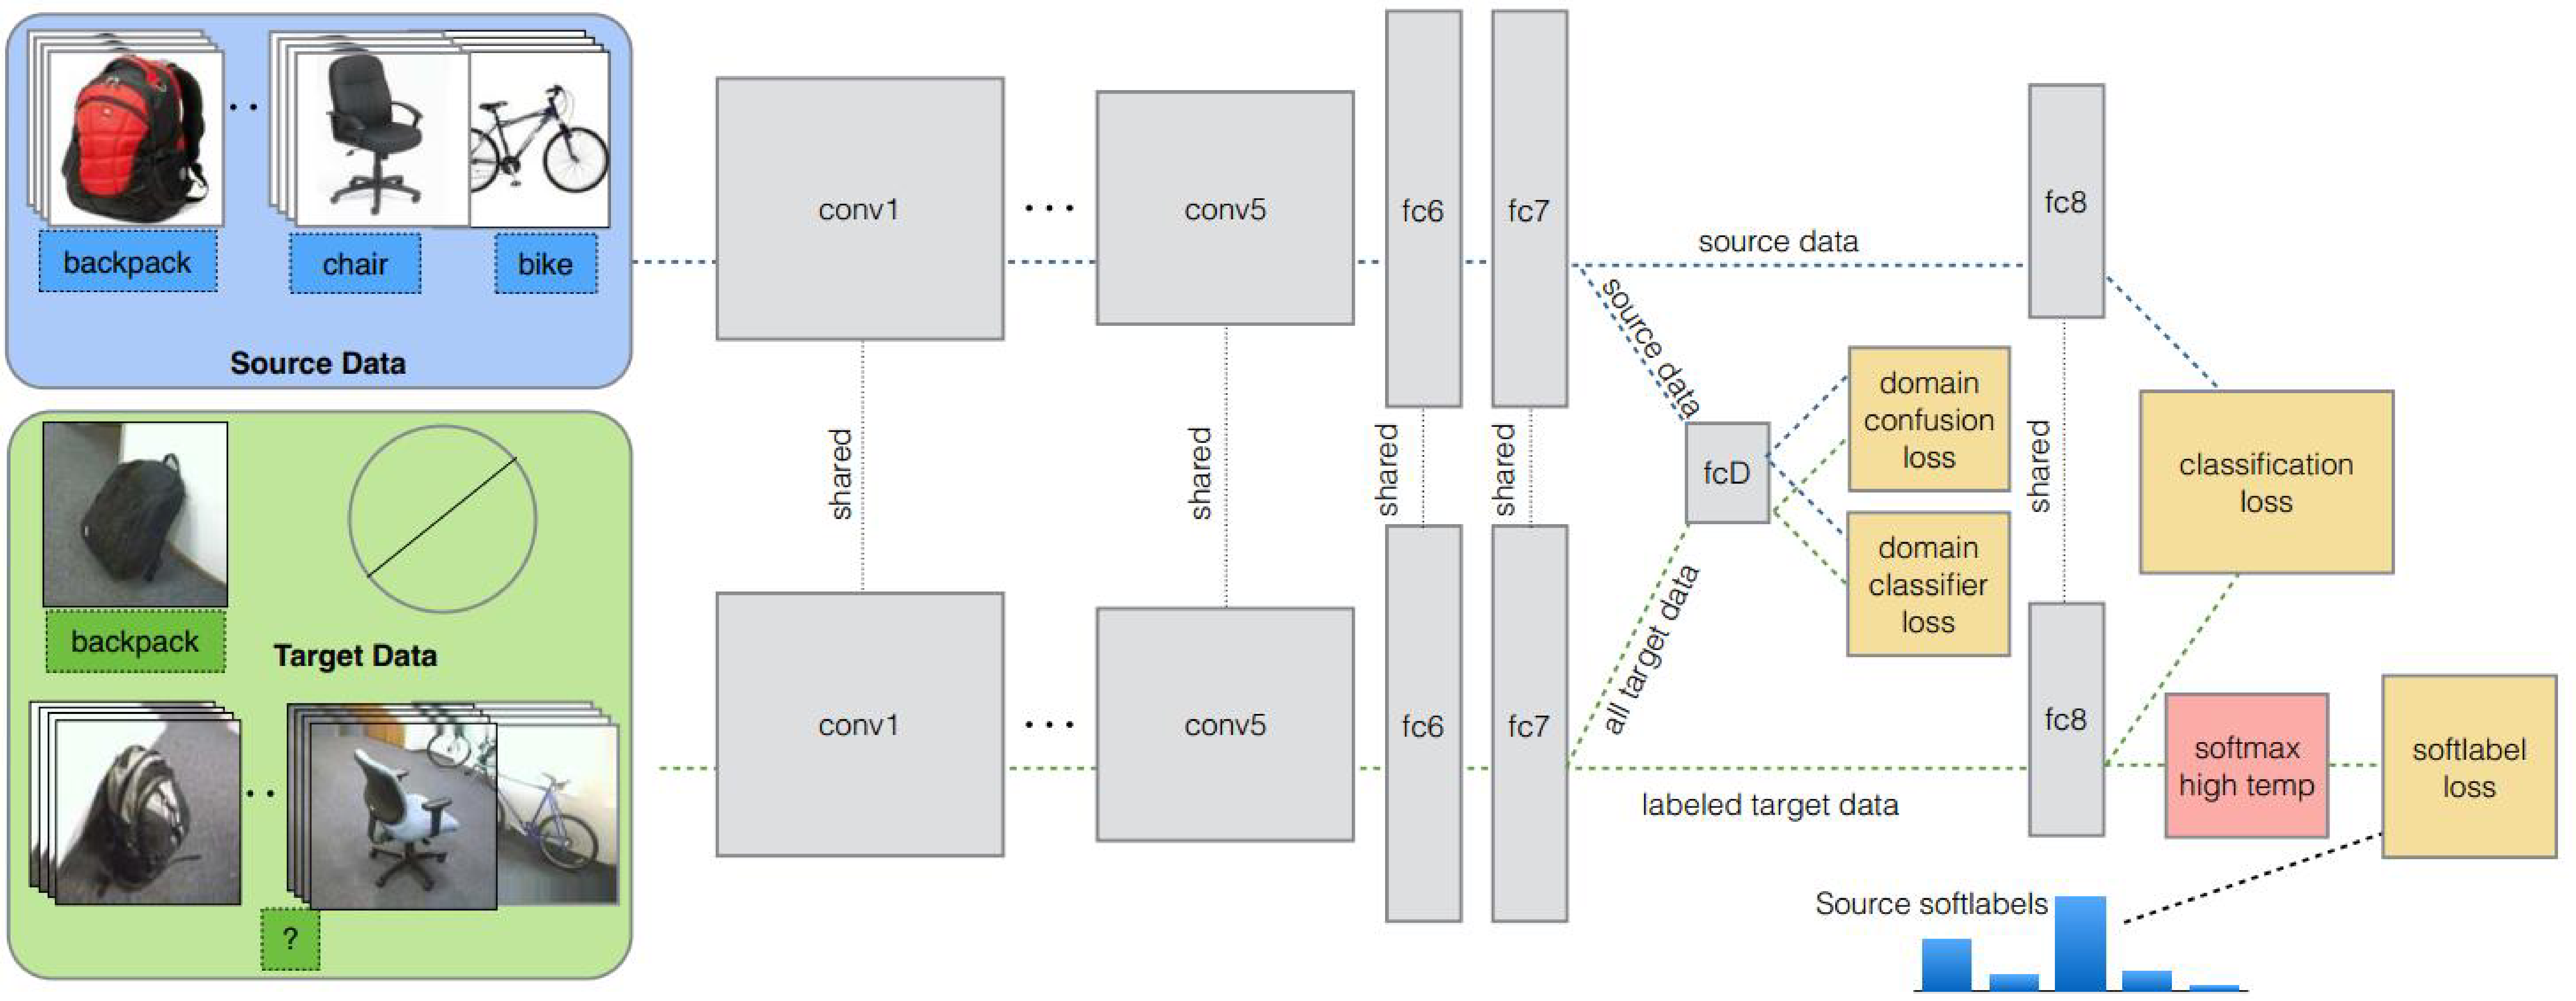
\includegraphics[scale=0.38]{./figures/fig-deep-tzeng2015.pdf}
	\caption{Joint CNN architecture for domain and task transfer方法示意图}
	\label{fig-deep-tzeng2015}
\end{figure}

Domain confusion就不用多说,和现有的一些比如DAN和JAN一样,直接对source和target的margina distribution进行估计即可。

什么是soft label loss?这和作者的motivation有关。不仅仅要适配两个domain的marginal distribution,也要把类别信息考虑进去。而target中有大量数据没有label,怎么办呢?可以利用source中的label信息。具体做法是:在网络对source进行训练的时候,把source的每一个样本处于每一个类的概率都记下来,然后,对于所有样本,属于每一个类的概率就可以通过求和再平均得到。如下图所示。这样的目的是:根据source中的类别分布关系,来对target做相应的约束。比如,source中和bike最相似的class,肯定是motorbike,而不是truck。这样有一定的道理。

但是在我看来,这就是深度网络版的conditional distribution adaptation。因为也对应于得到了每个类的proportion。只不过作者在这里取了个“soft label loss”这个好听的名字,再冠以“task transfer”这样高大上的名字。图~\ref{fig-deep-softlabel}是soft label的示意。

\begin{figure}[htbp]
	\centering
	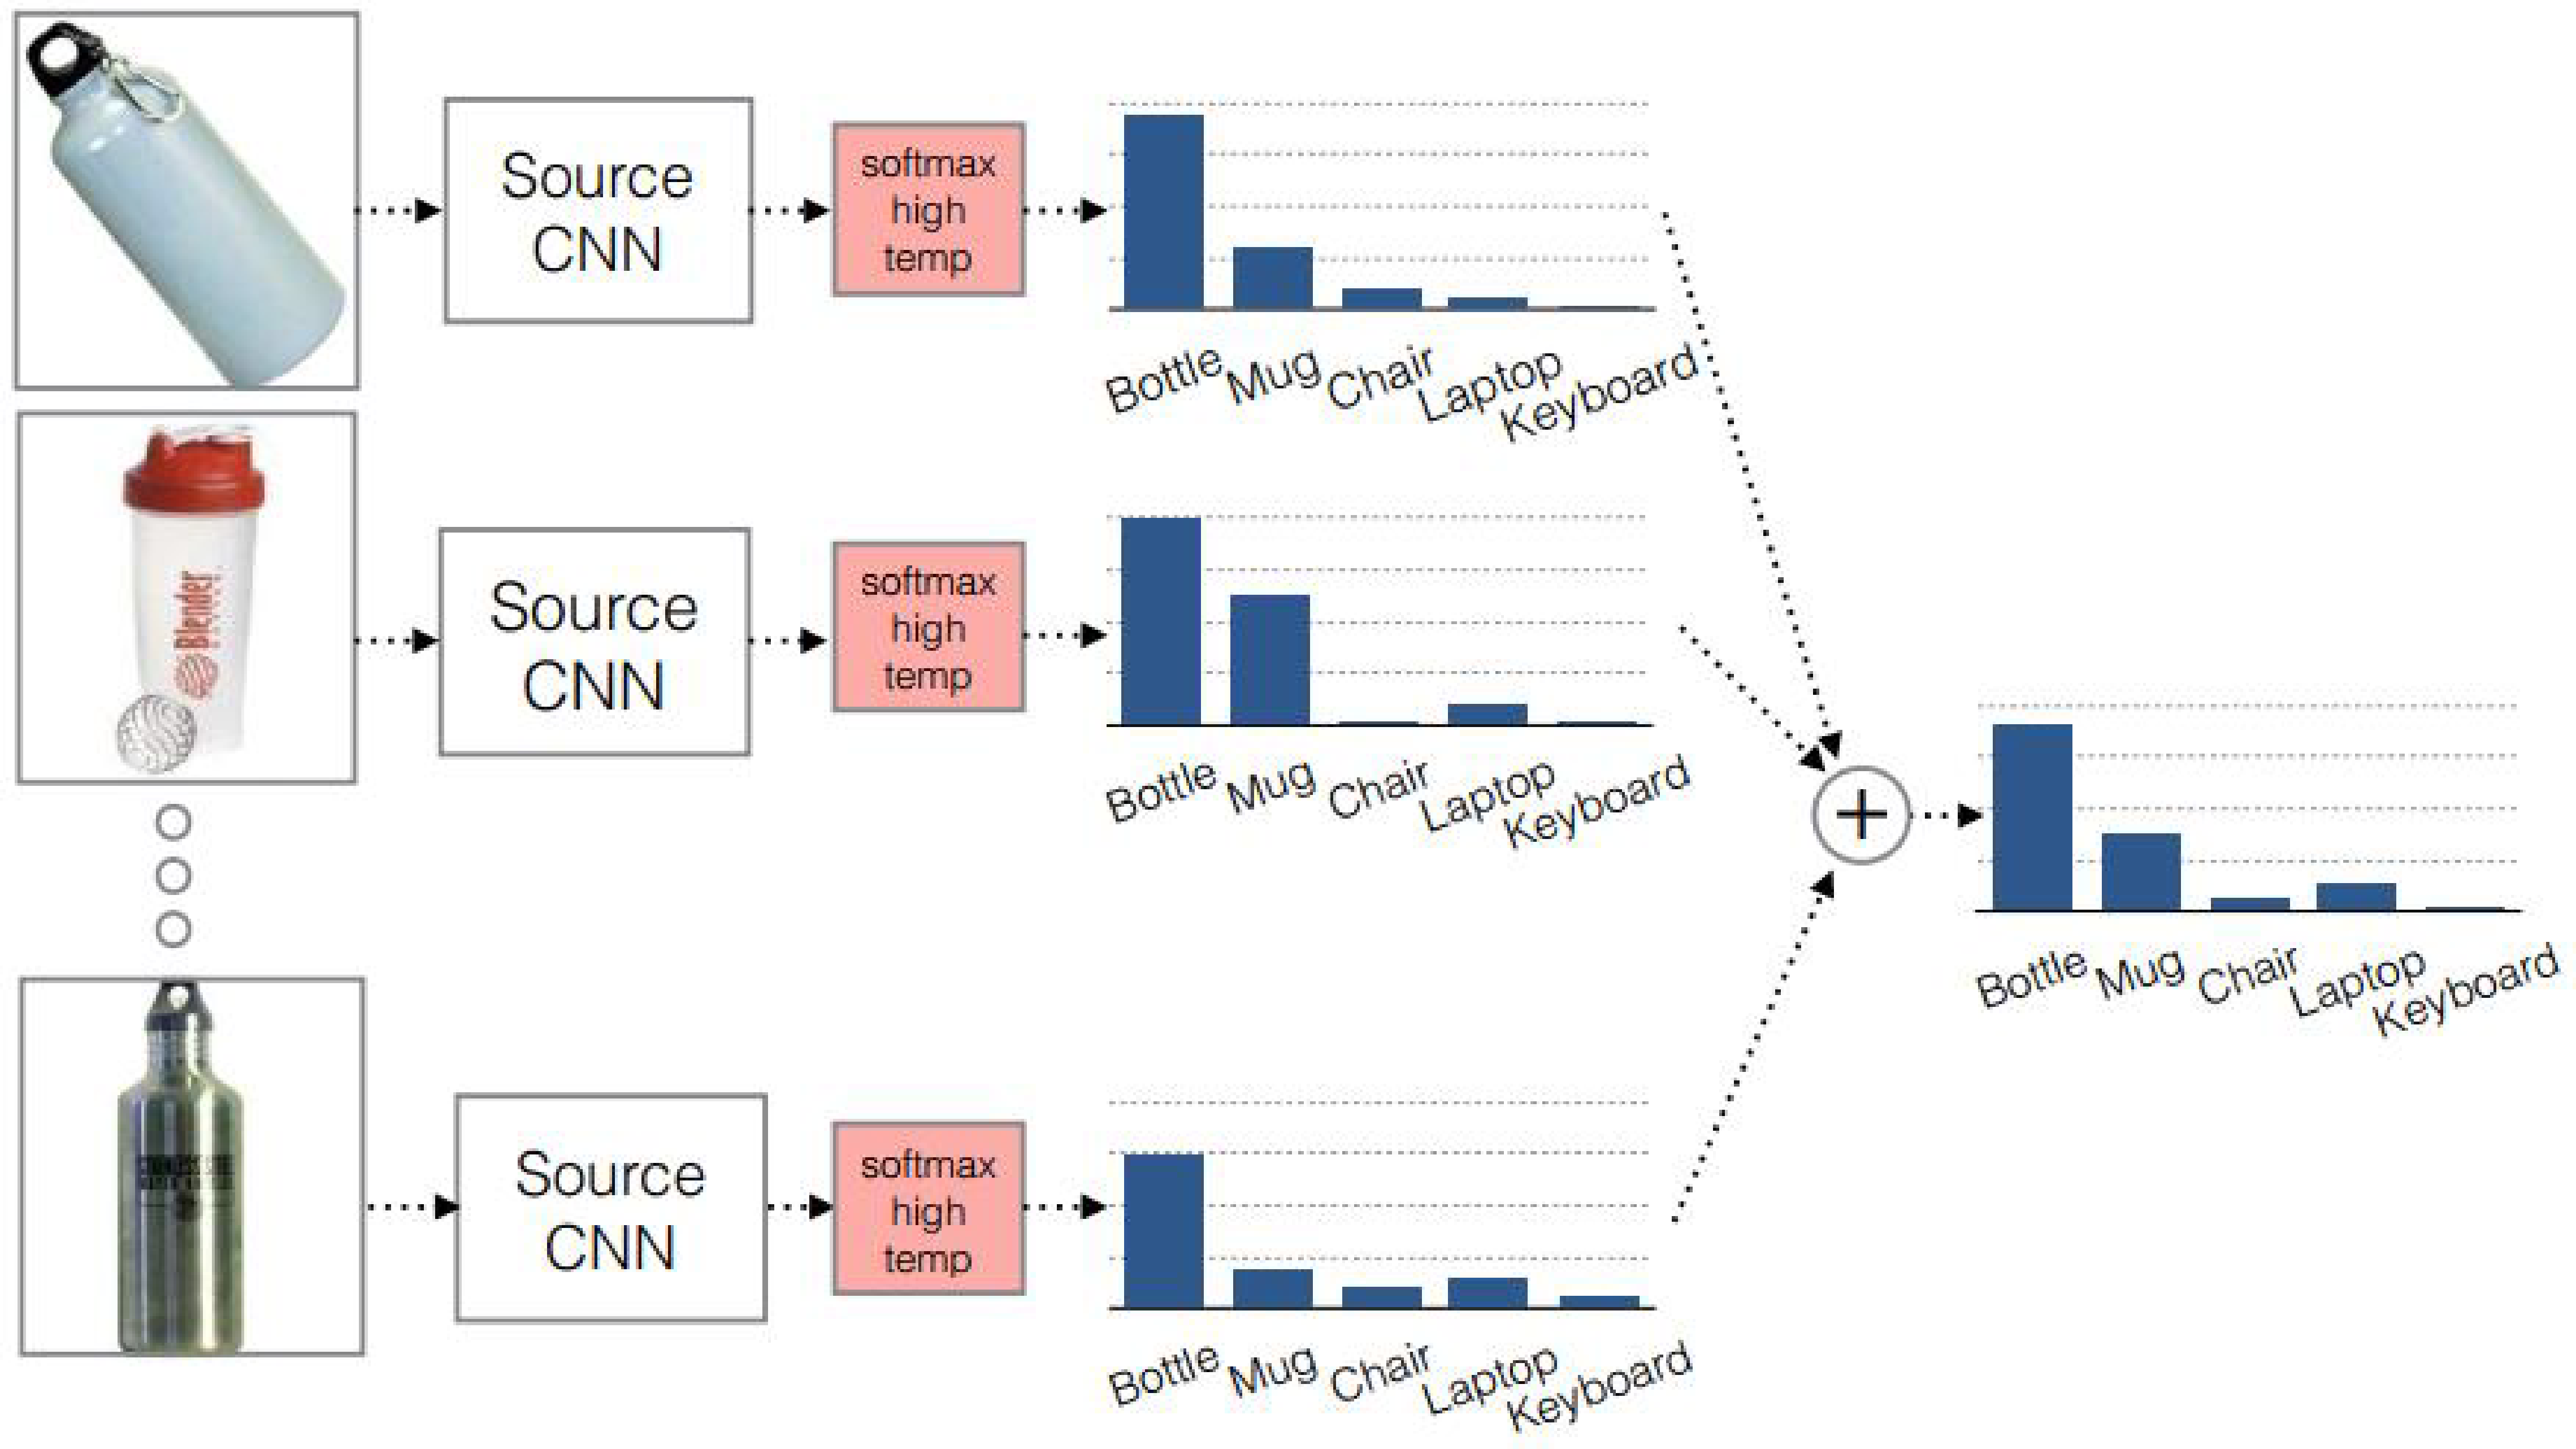
\includegraphics[scale=0.38]{./figures/fig-deep-softlabel.pdf}
	\caption{Softlabel示意图}
	\label{fig-deep-softlabel}
\end{figure}

\textbf{4. 深度联合分布自适应}

DAN的作者、清华大学的龙明盛在2017年机器学习顶级会议ICML上提出了JAN方法(Joint Adaptation Network)~\cite{long2017deep},在深度网络中同时进行联合分布的自适应和对抗学习。JAN方法将只对数据进行自适应的方式推广到了对类别的自适应,提出了JMMD度量(Joint MMD)。图~\ref{fig-deep-jan}是JAN的示意图。

\begin{figure}[htbp]
	\centering
	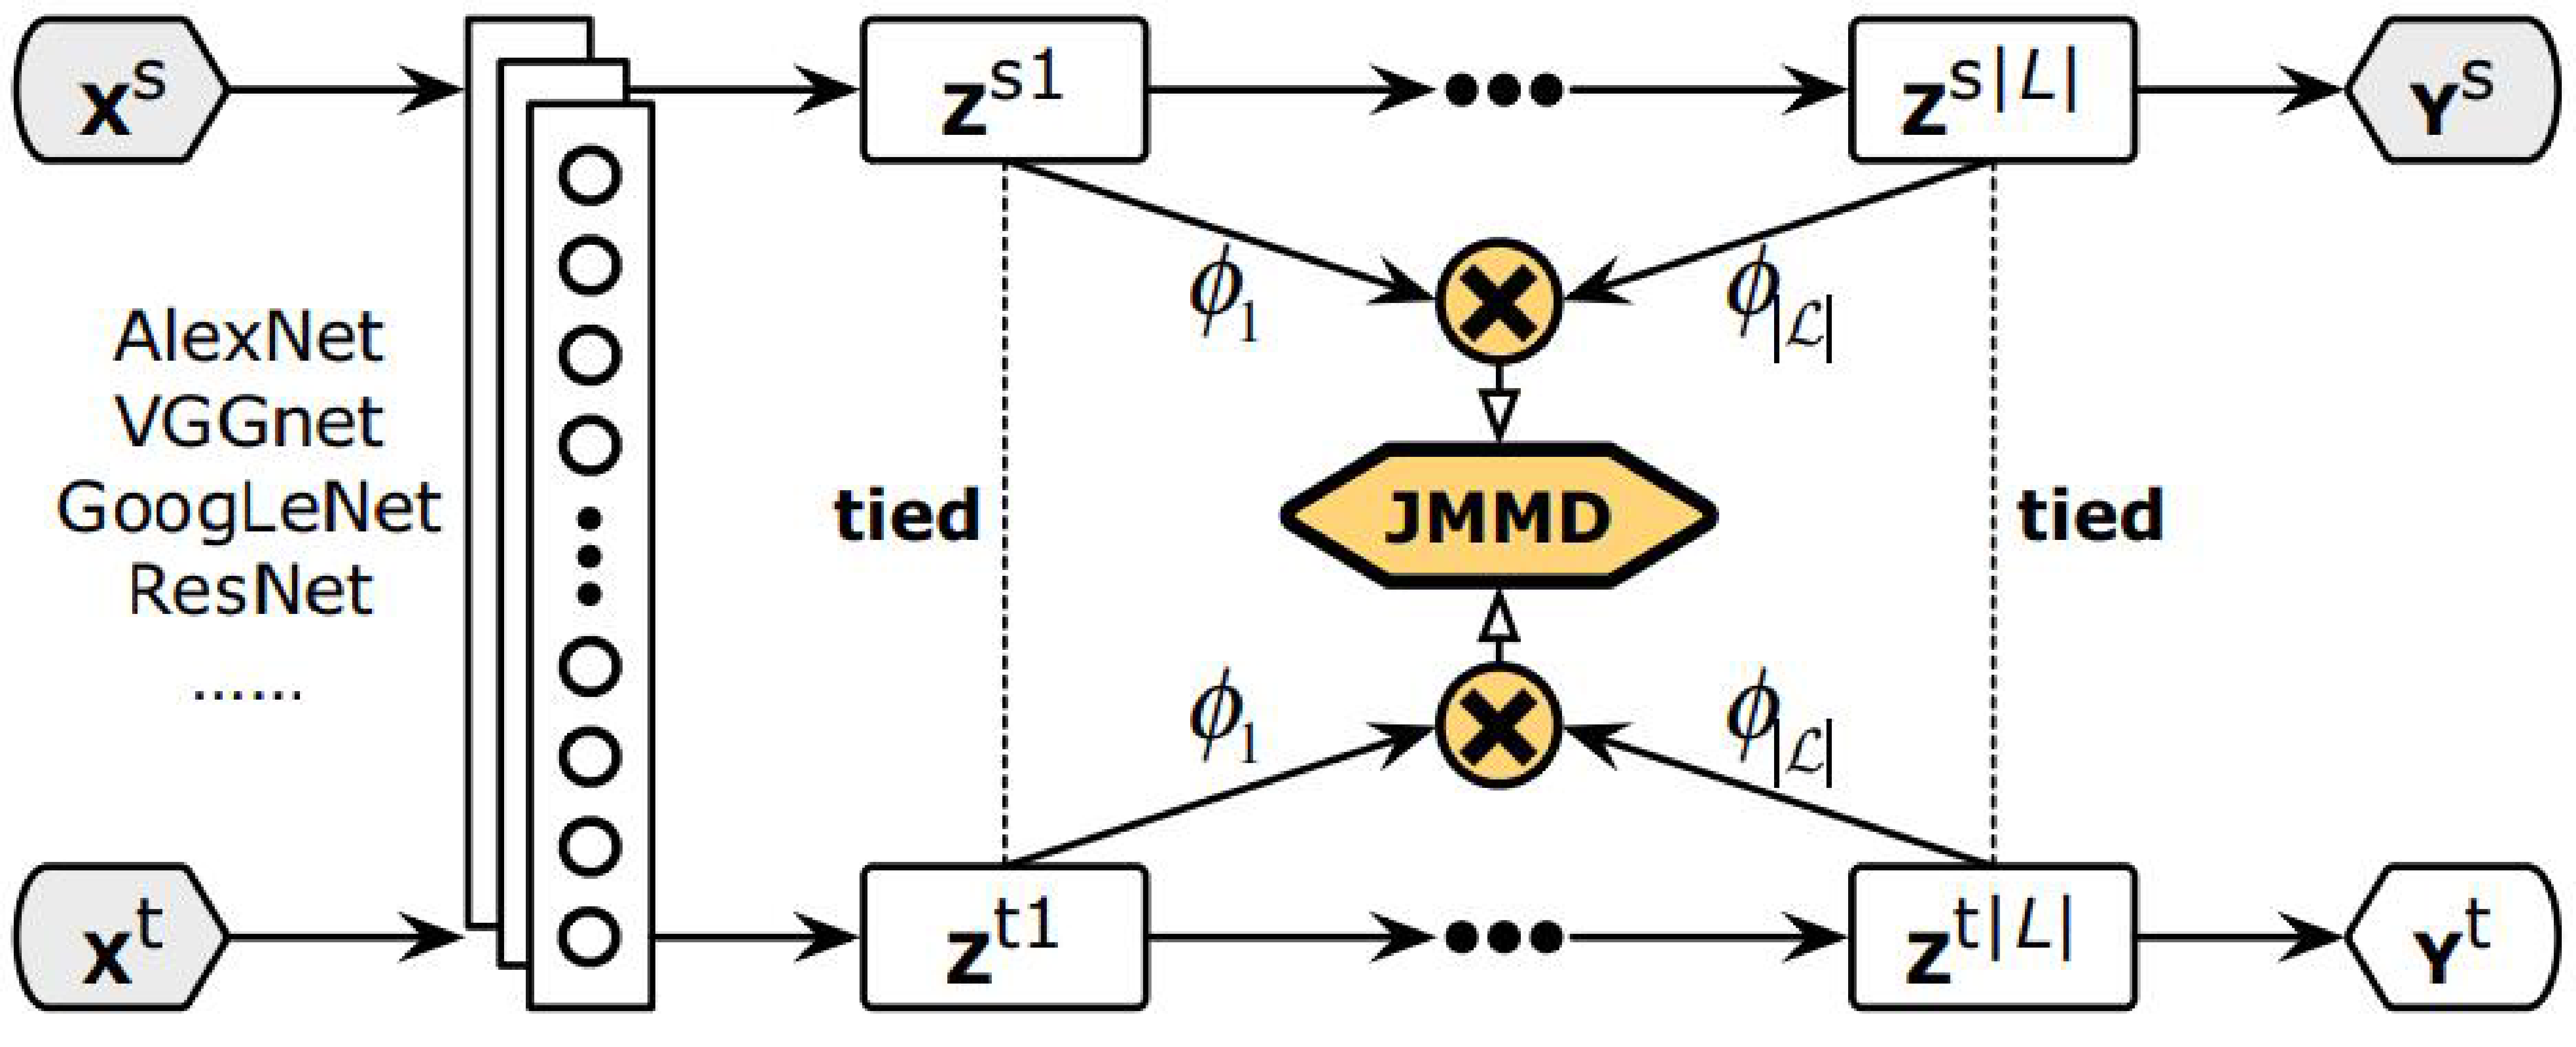
\includegraphics[scale=0.38]{./figures/fig-deep-jan.pdf}
	\caption{JAN方法示意图}
	\label{fig-deep-jan}
\end{figure}

\textbf{5. AdaBN}

与上述工作选择在已有网络层中增加适配层不同的是,北京大学的Haoyang Li和图森科技的Naiyan Wang等人提出了AdaBN(Adaptive Batch Normalization)~\cite{li2018adaptive},通过在归一化层加入统计特征的适配,从而完成迁移。

\begin{figure}[htbp]
	\centering
	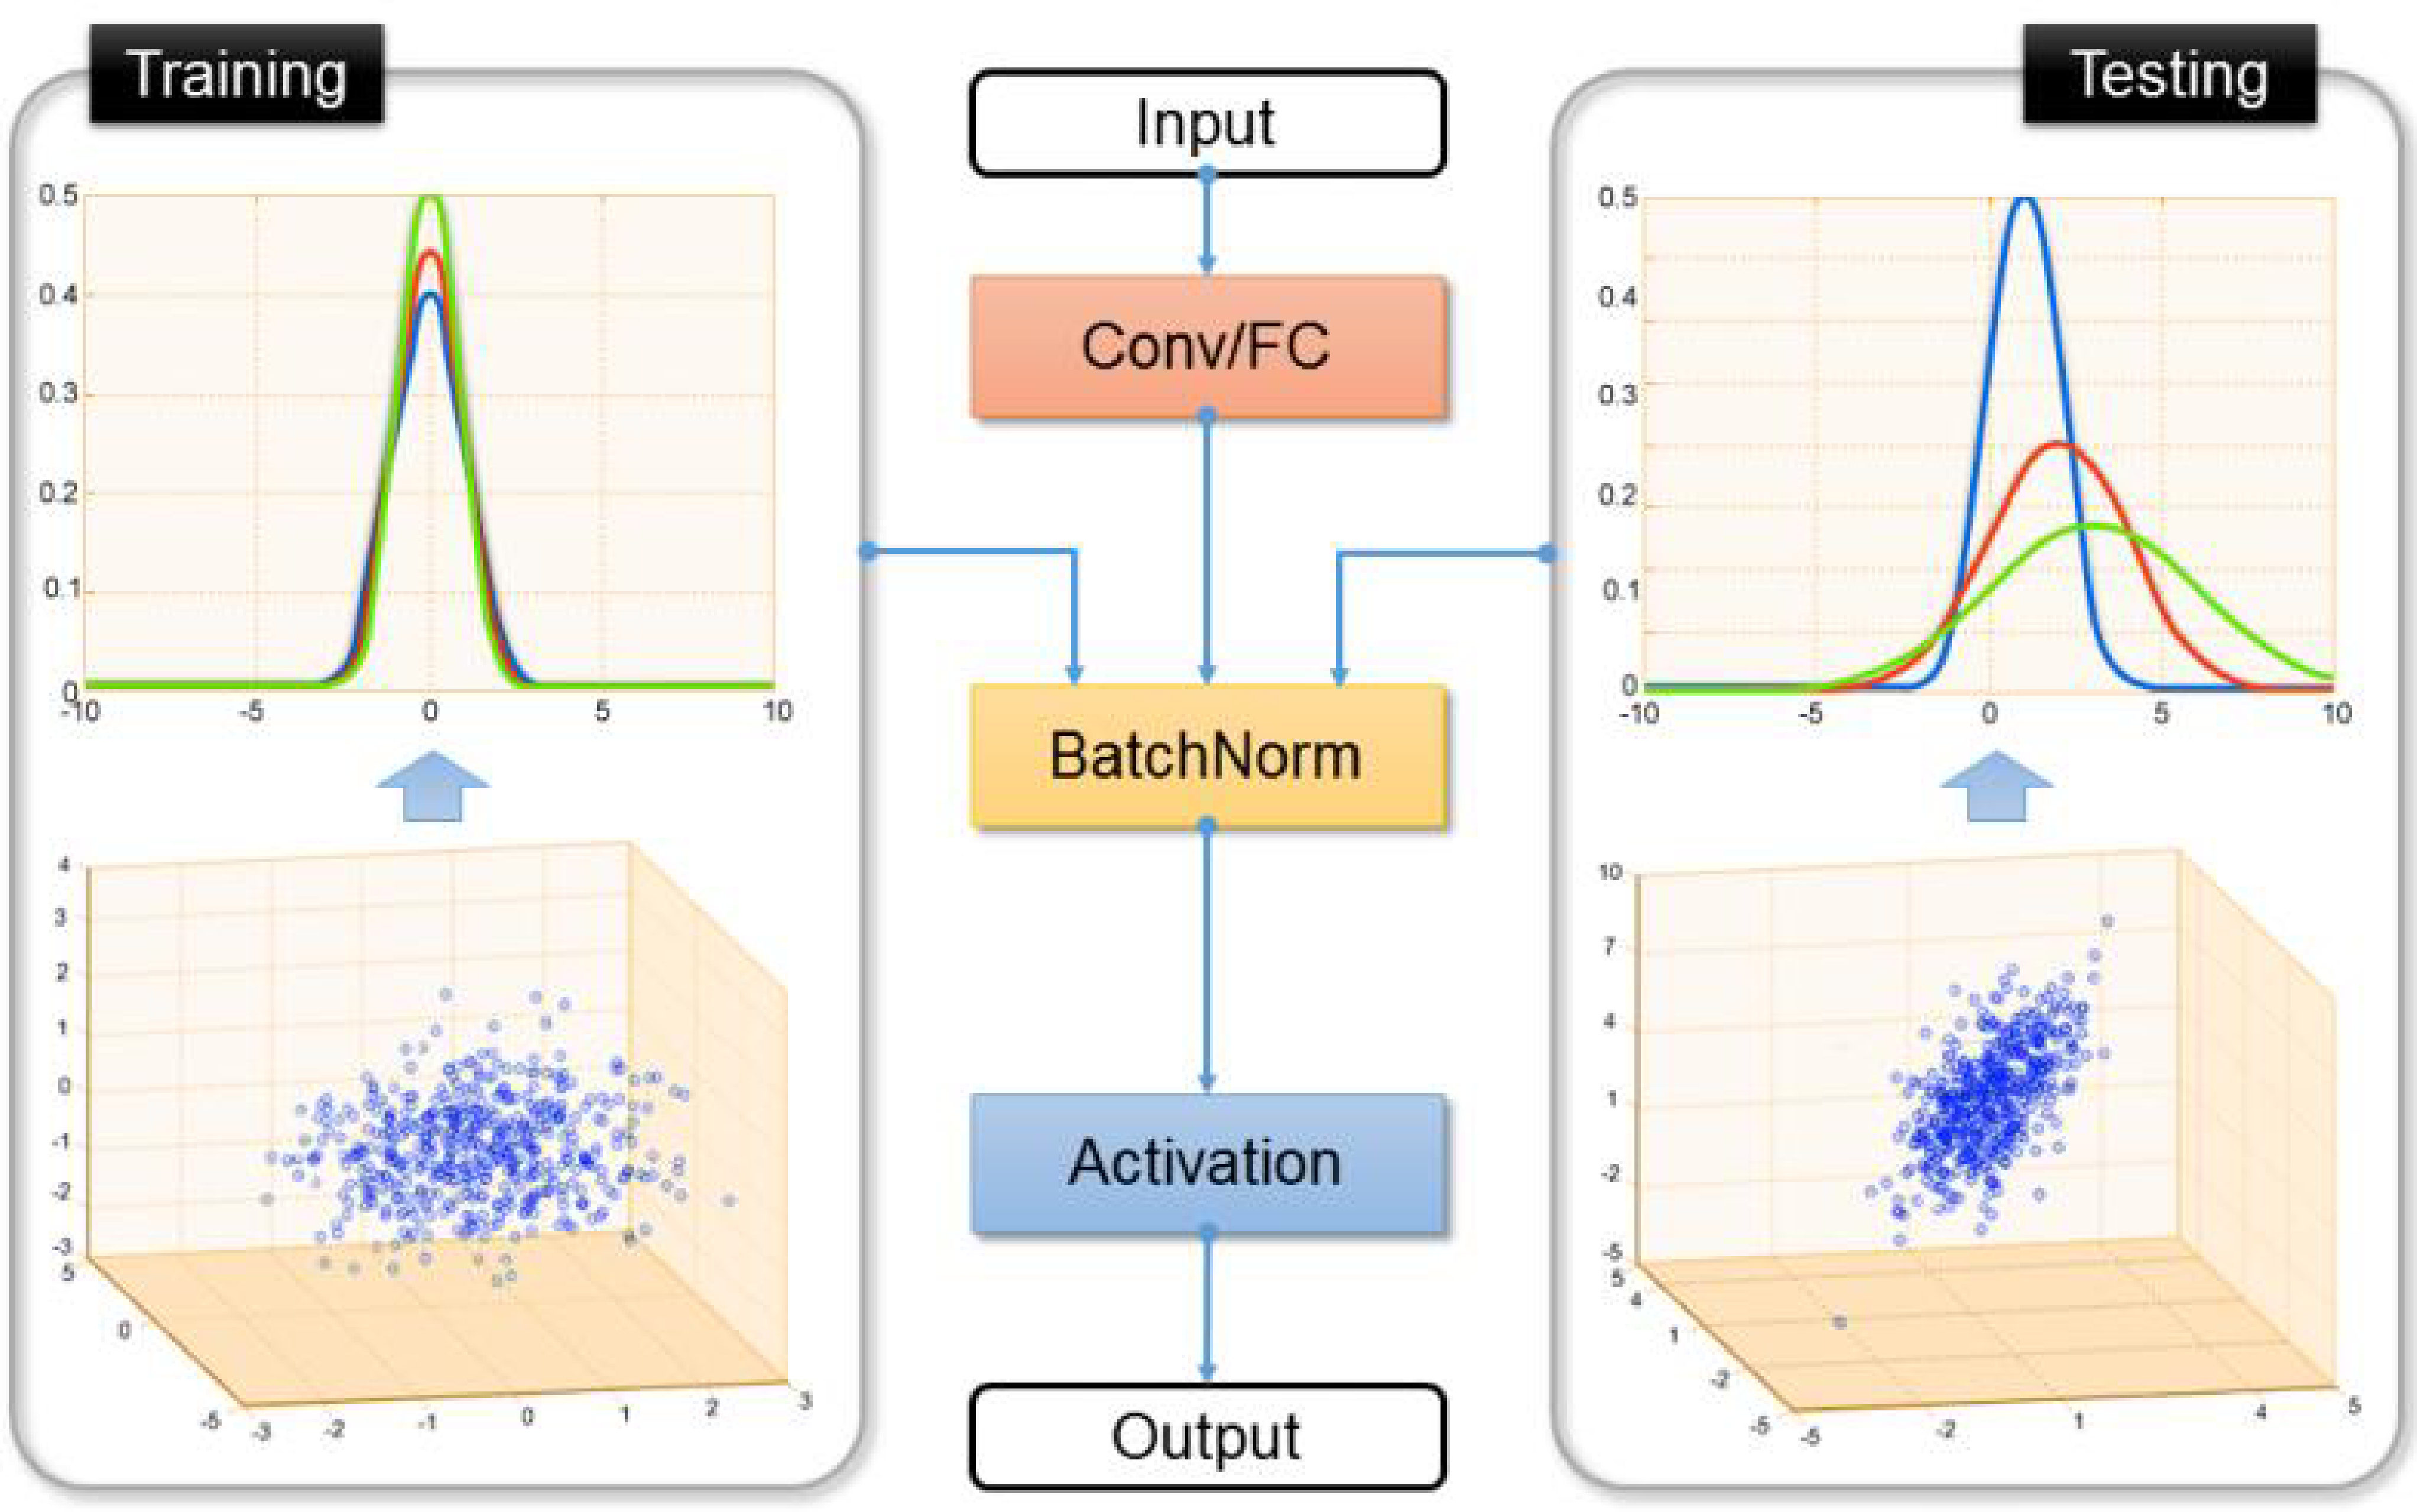
\includegraphics[scale=0.38]{./figures/fig-deep-adabn.pdf}
	\caption{AdaBN方法示意图}
	\label{fig-deep-adabn}
\end{figure}

AdaBN对比其他方法,实现相当简单。并且,方法本身不带有任何额外的参数。在许多公开数据集上都取得了很好的效果。

\subsubsection{小结}

基于深度网络进行迁移学习,其核心在于,找到网络需要进行自适应的层,并且对这些层加上自适应的损失度量。越来越多的研究者开始使用深度网络进行迁移学习~\cite{long2016deep,zhuo2017deep,zhuang2015supervised,sun2016deep,wei2016deep,luo2017label}。在这其中,几乎绝大多数方法都采用了卷积神经网络,在已训练好的模型(如AlexNet、Inception、GoogLeNet、Resnet等)上进行迁移。

特别地,最近意大利的学者Carlucci等人在2017年计算机视觉领域顶级会议ICCV上提出了自动深度网络自适应层(AutoDIAL, Automatic DomaIn Alignment Layers)~\cite{carlucci2017autodial}。该方法可以很简单地被加入现有的深度网络中,实现自动的自适应学习,使得深度网络的迁移更便捷。

由于篇幅和时间所限,我们未对所有新出现的研究工作给予介绍,仅在这里介绍了其中最具代表性的几种方法。但是绝大多数方法的原理都和我们已介绍过的大同小异。请读者持续关注最新发表的研究成果。

\subsection{深度对抗网络迁移}

生成对抗网络GAN(Generative Adversarial Nets)~\cite{goodfellow2014generative}是目前人工智能领域最炙手可热的概念之一。其也被深度学习领军人物Yann Lecun评为近年来最令人欣喜的成就。由此发展而来的对抗网络,也成为了提升网络性能的利器。本小节介绍深度对抗网络用于解决迁移学习问题方面的基本思路以及代表性研究成果。

\subsubsection{基本思路}

GAN受到自博弈论中的二人零和博弈(two-player game)思想的启发而提出。它一共包括两个部分:一部分为生成网络(Generative Network),此部分负责生成尽可能地以假乱真的样本,这部分被成为\textit{生成器}(Generator);另一部分为判别网络(Discriminative Network),此部分负责判断样本是真实的,还是由生成器生成的,这部分被成为\textit{判别器}(Discriminator)。生成器和判别器的互相博弈,就完成了对抗训练。

GAN的目标很明确:生成训练样本。这似乎与迁移学习的大目标有些许出入。然而,由于在迁移学习中,天然地存在一个源领域,一个目标领域,因此,我们可以免去生成样本的过程,而直接将其中一个领域的数据(通常是目标域)当作是生成的样本。此时,生成器的职能发生变化,不再生成新样本,而是扮演了特征提取的功能:不断学习领域数据的特征,使得判别器无法对两个领域进行分辨。这样,原来的生成器也可以称为特征提取器(Feature Extractor)。

通常用$G_f$来表示特征提取器,用$G_d$来表示判别器。

正是基于这样的领域对抗的思想,深度对抗网络可以被很好地运用于迁移学习问题中。

与深度网络自适应迁移方法类似,深度对抗网络的损失也由两部分构成:网络训练的损失$\ell_c$和领域判别损失$\ell_d$:

\begin{equation}
	\ell = \ell_c(\mathcal{D}_s,\mathbf{y}_s) + \lambda \ell_d(\mathcal{D}_s,\mathcal{D}_t)
\end{equation}

\subsubsection{核心方法}

\textbf{1. DANN}

Yaroslav Ganin等人~\cite{ganin2016domain}首先在神经网络的训练中加入了对抗机制,作者将他们的网络称之为DANN(Domain-Adversarial Neural Network)。在此研究中,网络的学习目标是:\textit{生成的特征尽可能帮助区分两个领域的特征,同时使得判别器无法对两个领域的差异进行判别}。该方法的领域对抗损失函数表示为:

\begin{equation}
	\ell_d = \max \left[-\frac{1}{n} \sum_{i=1}^{n} \mathcal{L}^i_d(\mathbf{W},\mathbf{b},\mathbf{u},z) - \frac{1}{n'} \sum_{i=n+1}^{N} \mathcal{L}^i_d(\mathbf{W},\mathbf{b},\mathbf{u},z)\right]
\end{equation}

其中的$\mathcal{L}_d$表示为

\begin{equation}
	\mathcal{L}_d(G_d(G_f(\mathbf{x}_i)),d_i) = d_i \log \frac{1}{G_d(G_f(\mathbf{x}_i))} + (1 - d_i) \log \frac{1}{G_d(G_f(\mathbf{x}_i))}
\end{equation}

\textbf{2. DSN}

来自Google Brain的Bousmalis等人通过提出DSN网络(Domain Separation Networks)~\cite{bousmalis2016domain}对DANN进行了扩展。DSN认为,源域和目标域都由两部分构成:公共部分和私有部分。公共部分可以学习公共的特征,私有部分用来保持各个领域独立的特性。DSN进一步对损失函数进行了定义:

\begin{equation}
	\ell = \ell_{task} + \alpha \ell_{recon} + \beta \ell_{difference} + \gamma \ell_{similarity}
\end{equation}

除去网络的常规训练损失$\ell_{task}$外,其他损失的含义如下:
\begin{itemize}
	\item $\ell_{recon}$: 重构损失,确保私有部分仍然对学习目标有作用
	\item $\ell_{difference}$: 公共部分与私有部分的差异损失
	\item $\ell_{similarity}$: 源域和目标域公共部分的相似性损失
\end{itemize}

图~\ref{fig-deep-dsn}是DSN方法的示意图。

\begin{figure}[htbp]
	\centering
	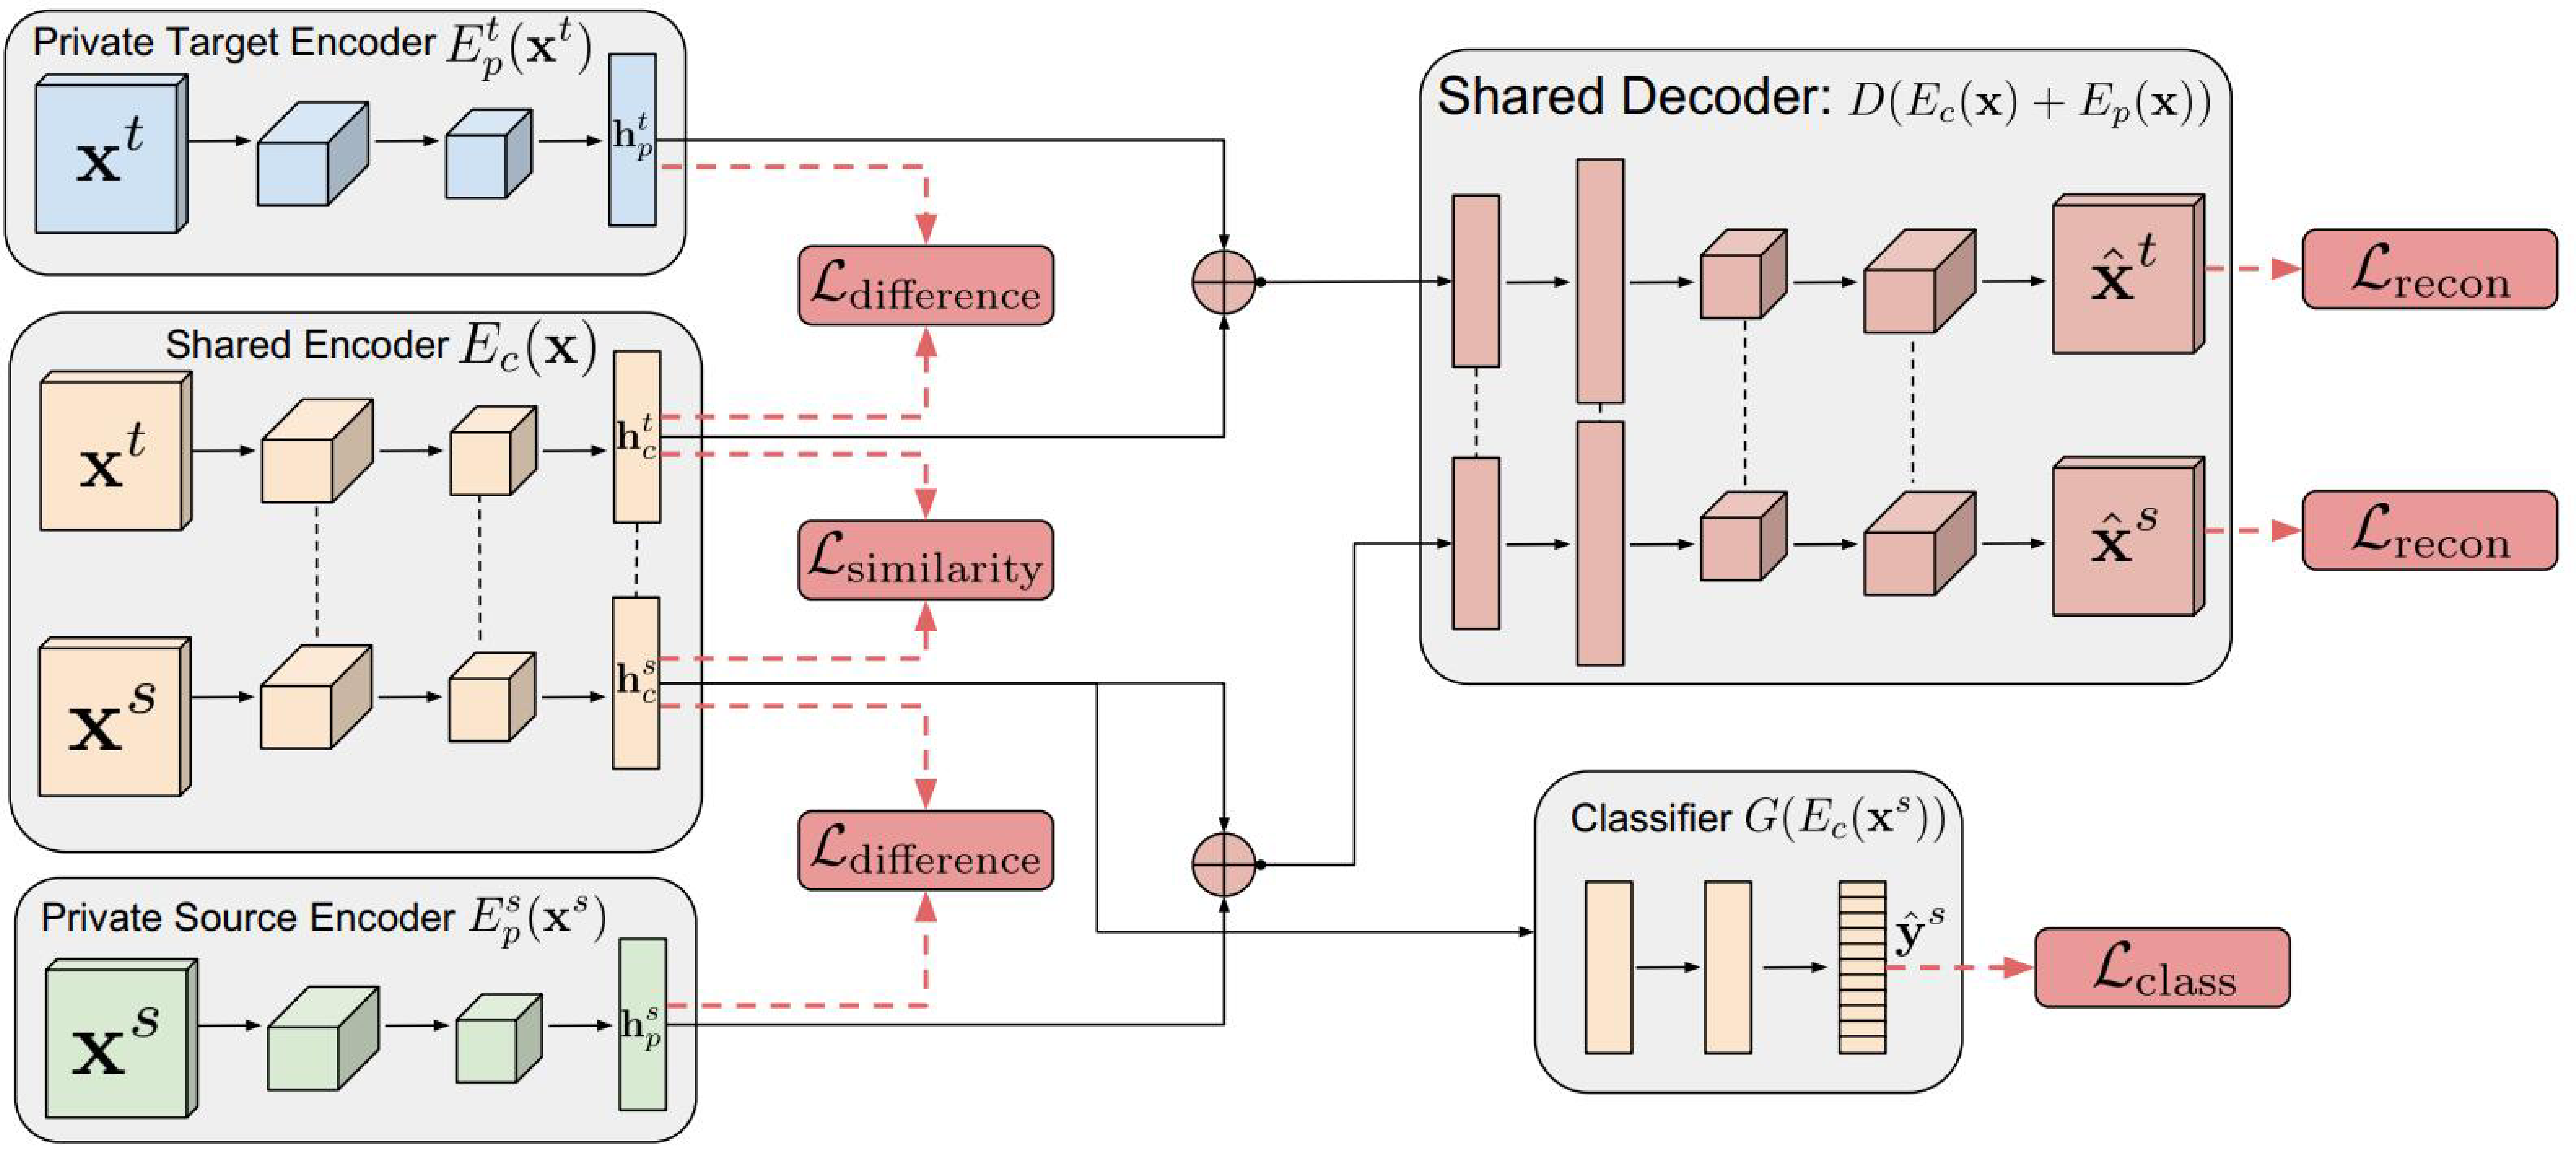
\includegraphics[scale=0.32]{./figures/fig-deep-dsn.pdf}
	\caption{DSN方法示意图}
	\label{fig-deep-dsn}
\end{figure}

DDC方法的作者、加州大学伯克利分校的Tzeng等人在2017年发表于计算机视觉顶级会议CVPR上的文章提出了ADDA方法(Adversarial Discriminative Domain Adaptation)~\cite{tzeng2017adversarial}。ADDA是一个通用的框架,现有的很多方法都可被看作是ADDA的特例。上海交通大学的研究者们用Wasserstein GAN进行迁移学习~\cite{shen2018w},Liu等人提出了Coupled GAN用于迁移学习~\cite{liu2016coupled}。这些工作都大体上按照之前思路进行。

\textbf{3. SAN}

清华大学龙明盛团队2018年发表在计算机视觉顶级会议CVPR上的文章提出了一个选择性迁移网络(Partial Transfer Learning)。作者认为,在大数据时代,通常我们会有大量的源域数据。这些源域数据比目标域数据,在类别上通常都是丰富的。比如基于ImageNet训练的图像分类器,必然是针对几千个类别进行的分类。我们实际用的时候,目标域往往只是其中的一部分类别。这样就会带来一个问题:那些只存在于源域中的类别在迁移时,会对迁移结果产生负迁移影响。

这种情况通常来说是非常普遍的。因此,就要求相应的迁移学习方法能够对目标域,选择相似的源域样本(类别),同时也要避免负迁移。但是目标域通常是没有标签的,不知道和源域中哪个类别更相似。作者指出这个问题叫做partial transfer learning。这个partial,就是只迁移源域中那部分和目标域相关的样本。图~\ref{fig-deep-partial}展示了部分迁移学习的思想。

\begin{figure}[htbp]
	\centering
	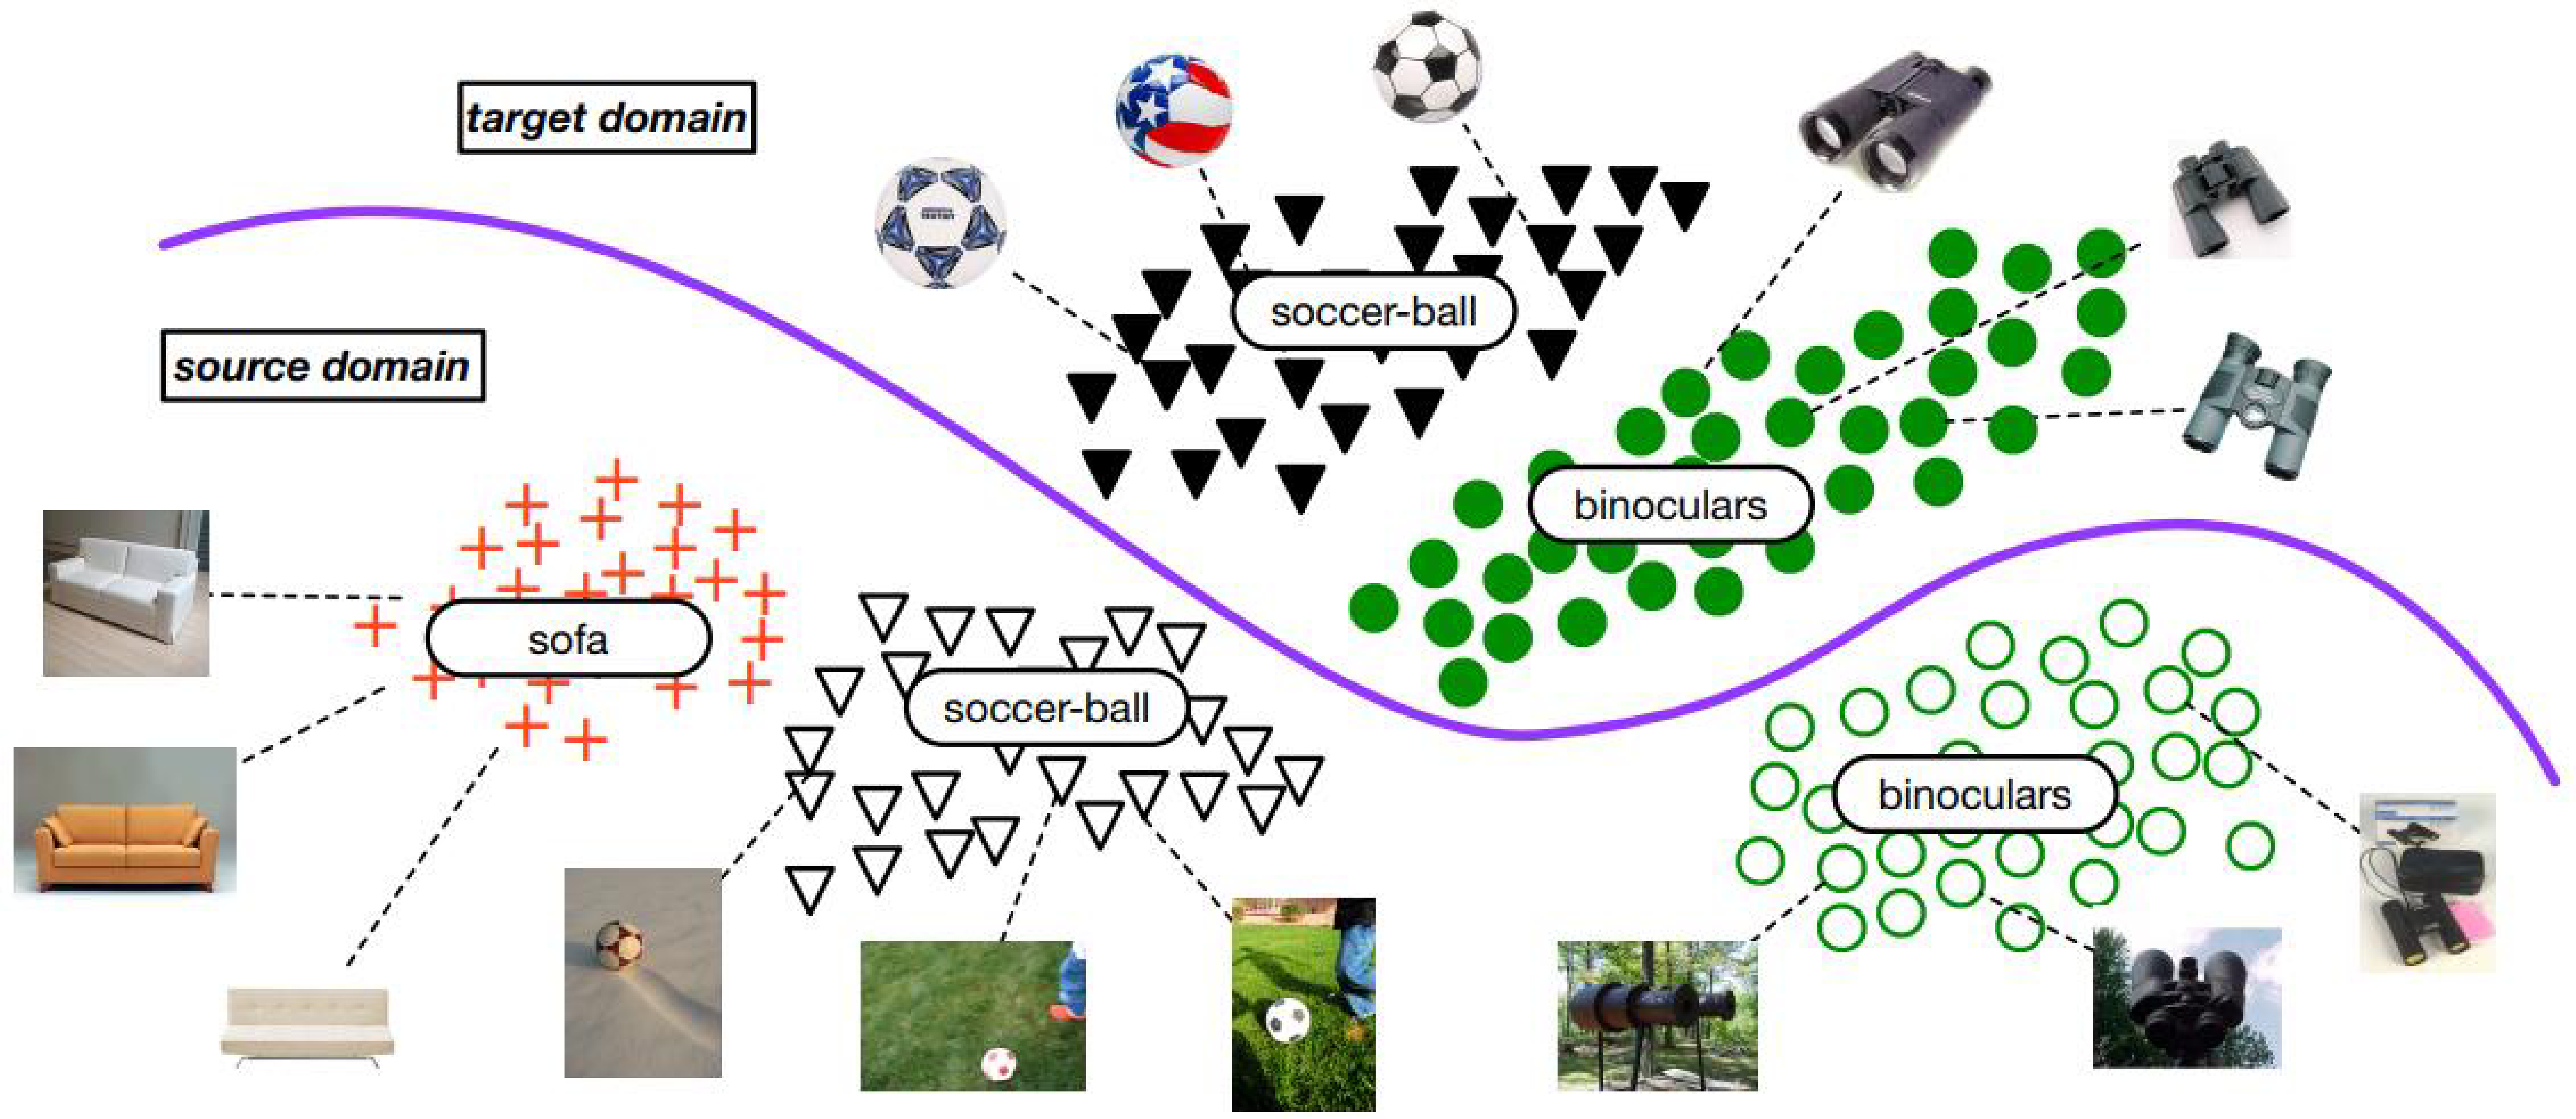
\includegraphics[scale=0.32]{./figures/fig-deep-partial.pdf}
	\caption{部分迁移学习示意图}
	\label{fig-deep-partial}
\end{figure}

作者提出了一个叫做Selective Adversarial Networks (SAN)~\cite{cao2017partial}的方法来处理partial transfer问题。在partial问题中,传统的对抗网络不再适用。所以就需要对进行一些修改,使得它能够适用于partial问题。

因为不知道目标域的标签,也就没办法知道到底是源域中哪些类是目标域的。为了达到这个目的,作者对目标域按照类别分组,把原来的一整个判别器分成了$|\mathcal{C}_s|$个:$G^k_d$,每一个子判别器都对它所在的第$k$个类进行判别。作者观察到了这样的事实:对于每个数据点$\mathbf{x}_i$来说,分类器的预测结果 $\hat{\mathbf{y}}_i$ 其实是对于整个类别空间的一个\textit{概率分布}。因此,在进行对抗时,需要考虑每个样本属于每个类别的影响。这个影响就是由概率来刻画。所以作者提出了一个概率权重的判别器:

\begin{equation}
	L'_d=\frac{1}{n_s+n_t} \sum_{k=1}^{|\mathcal{C}_s|} \sum_{\mathbf{x}_i \in \mathcal{D}_s + \mathcal{D}_t}^{} \hat{y}^k_i L^k_d(G^k_d(G_f(\mathbf{x}_i)),d_i)
\end{equation}

上面这个式子能很好地在partial transfer情景下,避免负迁移。这种约束是样本级别的,就是可以控制尽可能让更相似的样本参与迁移。除此之外,作者还介绍了一个类别级别的约束,可以很好地避免不在目标域中的那些类别不参与迁移。于是,进一步地,变成了下面的约束

\begin{equation}
	L'_d=\frac{1}{n_s+n_t} \sum_{k=1}^{|\mathcal{C}_s|} \sum_{\mathbf{x}_i \in \mathcal{D}_s + \mathcal{D}_t}^{} (\frac{1}{n_t} \sum_{\mathbf{x}_i^{} \in \mathcal{D}_t}\hat{y}^k_i) L^k_d(G^k_d(G_f(\mathbf{x}_i)),d_i)
\end{equation}

上面这个式子比较依赖于之前说的每个样本的预测概率。为了消除这个影响,作者又在目标域上加了一项熵最小化

\begin{equation}
	E=\frac{1}{n_t} \sum_{\mathbf{x}_i \in \mathcal{D}_t} H(G_y(G_f(\mathbf{x}_i)))
\end{equation}

\textbf{4. DAAN}

最近,Yu等人在~\cite{yu2019transfer}中将动态分布适配的概念进一步扩展到了对抗网络中,证明了对抗网络中同样存在边缘分布和条件分布不匹配的问题。作者提出一个动态对抗适配网络DAAN (Dynamic Adversarial Adaptation Networks)来解决对抗网络中的动态分布适配问题,取得了当前的最好效果。图~\ref{fig-deep-daan}展示了DAAN的架构。

\begin{figure}[htbp]
	\centering
	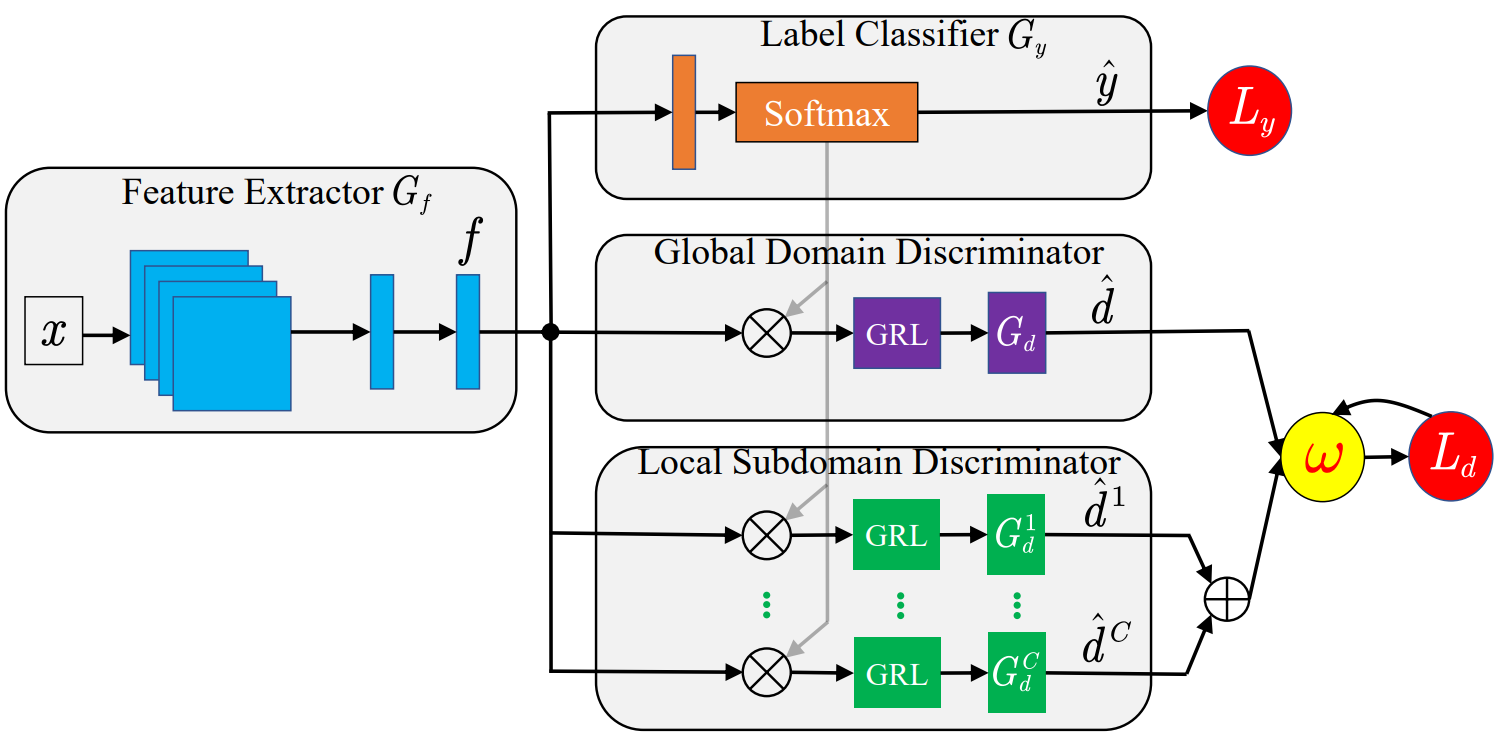
\includegraphics[scale=.35]{./figures/fig-distribution-daan.png}
	\caption{动态对抗适配网络DAAN结构示意图}
	\label{fig-deep-daan}
\end{figure}

\subsubsection{小结}

使用对抗网络进行迁移学习是近年来的研究热点。我们期待在这个领域会有越来越多的工作发表。